\documentclass[journal]{IEEEtran}

%% ─── Packages ────────────────────────────────────────────────────────────────
\usepackage{cite}
\usepackage{amsmath,amssymb,amsfonts}
\usepackage{algorithmic}
\usepackage{algorithm}
\usepackage{graphicx}
\usepackage{textcomp}
\usepackage{xcolor}
\usepackage{hyperref}
\usepackage{booktabs}
\usepackage{multirow}
\usepackage{array}
\usepackage{url}
\usepackage{bm}

% Tracked-revision convention required for this working manuscript.
\newcommand{\added}[1]{\textcolor{blue}{#1}}
\newcommand{\todo}[1]{\textcolor{green!50!black}{\textbf{TODO:\{#1\}}}}

\hypersetup{
    colorlinks=true,
    linkcolor=blue,
    citecolor=blue,
    urlcolor=blue
}

\def\BibTeX{{\rm B\kern-.05em{\sc i\kern-.025em b}\kern-.08em
    T\kern-.1667em\lower.7ex\hbox{E}\kern-.125emX}}

% NOTE TO AUTHORS: switched from [conference] to [journal] class option, and
% from conference-style \IEEEauthorblockN/\IEEEauthorblockA to the standard
% journal author/affiliation format (with \thanks footnotes), since IEEE
% Transactions on Reliability is a journal, not a conference proceedings venue.

% ─── Document ────────────────────────────────────────────────────────────────
\begin{document}

\title{A Multi-Architecture Neural Operator Digital Twin: A Proof-of-Concept Surrogate Methodology for Cold-Leg LOCA Screening in AP1000 Nuclear Reactors}

\author{Punyansh~Thakur, Anushka~Paul, Ayush~Kumar~Bhadra, and~Vinay~Kumar
\thanks{P. Thakur, A. Paul, A. K. Bhadra, and V. Kumar are with the Department of Computer Science and Engineering, IIIT Naya Raipur, India (e-mail: punyansh24102@iiitnr.edu.in; anushka24102@iiitnr.edu.in; ayush24101@iiitnr.edu.in; vinay@iiitnr.edu.in). Corresponding author: V. Kumar.}}

\markboth{IEEE Transactions on Reliability,~Vol.~XX, No.~XX, 2026}%
{Thakur \MakeLowercase{\textit{et al.}}: A Multi-Architecture Neural Operator Digital Twin for Cold-Leg LOCA Screening in AP1000 Nuclear Reactors}

\maketitle

%─── Abstract ─────────────────────────────────────────────────────────────────
\begin{abstract}

\added{High-fidelity computational-fluid-dynamics (CFD) analysis is too costly for high-throughput Cold-Leg Loss-of-Coolant Accident (LOCA) screening. This paper presents a proof-of-concept AP1000 digital-twin methodology evaluated on 2,000 analytically generated, physics-consistent synthetic cases, not on validated Fluent or plant-transient data. Three neural operators map inlet velocity, prescribed break size, and coolant temperature to pressure, velocity magnitude, turbulent kinetic energy, and temperature on a shared 25,000-node mesh: DeepONetFourier (1,451,012 parameters), Transolver++ (3,244,872), and a grade-structured Clifford operator (37,380). DeepONetFourier combines random Fourier features and adaptive GELU activations with two serialized-node regularizers. Because the stored targets contain velocity magnitude rather than velocity components, these terms are index-space smoothness proxies and are not physical spatial-gradient or mass-conservation constraints. On the 300-case held-out synthetic test set, the archived DeepONetFourier checkpoint achieved pooled $R^2$ values of 0.9961, 0.9958, 0.9951, and 0.9962 for pressure, velocity magnitude, turbulent kinetic energy, and temperature, respectively. Its loss differs from the MSE-only Transolver++ and Clifford training objectives; therefore, the architecture comparison is not controlled. A gradient-boosting classifier trained on open PCTRAN-simulated NPPAD records plus synthetic transition samples achieved ROC-AUC 0.990554 and recall 0.989063 on one fixed split. A five-seed translation-path ablation retained high ROC-AUC after removing the translator's explicit break-severity blend, but prescribed break size remained an operator input assigned from the class label; the result is consequently a pipeline-consistency demonstration, not independent LOCA detection. Reported end-to-end latency is below 20\,ms. The corresponding $\sim$180,000$\times$ figure uses 3,600\,s as a conservative assumed lower bound for a 1--4\,h Fluent case and is not a matched CFD timing experiment. The results support synthetic-benchmark feasibility only; full-fidelity CFD validation, label-independent detection tests, matched-loss multi-seed comparisons, and reliability-oriented operating-point analysis remain prerequisites for safety-relevant claims.}
\end{abstract}

\begin{IEEEkeywords}
Digital Twin, DeepONet, Transolver, Clifford Neural Operator, Geometric Algebra, Transformer Neural Operator, LOCA, AP1000, Nuclear Safety, CFD Surrogate, Fourier Feature Encoding
\end{IEEEkeywords}

%═══════════════════════════════════════════════════════════════════════════════
\section{Introduction}
%═══════════════════════════════════════════════════════════════════════════════

The AP1000 is a Generation~III+ pressurized water reactor (PWR) designed by the Westinghouse Electric Company, featuring 1,000\,MWe output and passive safety systems. A Cold-Leg Loss-of-Coolant Accident (LOCA)---a rupture in the primary coolant return piping---is a design-basis event that demands rapid detection to prevent core uncovery and fuel damage \cite{wecdcd}. Traditional safety monitoring relies on threshold-based single-sensor alarms, which respond slowly to incipient partial breaks and can miss the early stages of a developing event before critical parameters are exceeded \cite{nrc_loca}.

High-fidelity CFD simulations (e.g., ANSYS Fluent) can predict the complete thermohydraulic state but require 1--4 hours per scenario, making real-time deployment infeasible. Neural operators---machine learning models that learn mappings between infinite-dimensional function spaces---have emerged as powerful Partial Differential Equation (PDE) surrogates. Lu et al.~\cite{lu2021deeponet} introduced Deep Operator Networks (DeepONet), decomposing the solution operator $\mathcal{G}: \mathcal{U} \to \mathcal{V}$ via a branch-trunk factorization. The baseline DeepONet architecture, however, suffers from well-documented limitations: \emph{spectral bias} causing poor resolution of sharp gradients \cite{rahaman2019spectral} and fixed ReLU activations that cannot adapt their slope during training.  \added{The present implementation instead adds serialized-node smoothness proxies; Section~\ref{sec:deeponet_fourier} defines their scope explicitly. The $\sim$180,000$\times$ speedup reported later divides a conservative assumed 3,600\,s lower-bound Fluent runtime by a sub-20\,ms pipeline latency. It is a reference-ratio estimate, not a matched timing measurement.} \todo{Measure Fluent and surrogate latency on matched hardware with an identical timing boundary, then replace the reference-ratio estimate.}

Subsequent work has explored alternative neural operator paradigms: Transolver~\cite{wu2024transolver} applies transformer attention to mesh-compressed tokens for general-geometry PDE solving, and Clifford Neural Operators~\cite{brandstetter2023clifford} use geometric-algebra representations to encode grade structure.  \added{A targeted public-source search through August~2026 found no directly matching report that evaluates both Transolver- and Clifford-style operators in a Cold-Leg LOCA surrogate-to-classifier workflow. This is a qualified search result, not proof of absence from the complete literature.} \todo{Repeat and document the final novelty search in Scopus and Web of Science immediately before submission, including query strings, date range, and screened records.}

The Fourier Neural Operator (FNO) \cite{li2021fno} is a natural candidate for comparison; however, the fixed structured AP1000 cold-leg geometry and the low-dimensional parametric input ($v, b, T$) motivated branch--trunk operator learning as the primary architectural comparison focus in this initial study. FNO comparison under appropriate structured-grid conditions is reserved for future controlled benchmarking.

The main contributions of this paper are summarized as follows:
\begin{enumerate}
    \item We design and implement three neural operator architectures---upgraded DeepONetFourier, Transolver++, and Clifford Neural Operator---within a unified proof-of-concept digital twin pipeline for LOCA screening, each addressing a distinct limitation of the baseline DeepONet.
    \item We introduce four changes to baseline DeepONet---random Fourier feature encoding ($\sigma = 10.0$, $m = 256$), per-neuron adaptive GELU activations, an index-gradient matching term ($\beta = 0.1$), and a velocity-variation term ($\lambda = 0.01$)--- \added{reducing the measured parameter count from 3,162,116 to 1,451,012 (54.1\%)} under the synthetic benchmark. \added{The latter two terms are serialized-node regularizers rather than geometry-aware physics derivatives.}
    \item We evaluate Transolver++ (mesh-token attention with $M = 64$ tokens, 3,244,872 parameters) and a grade-structured Clifford operator (37,380 parameters) as reactor flow-field surrogates.  \added{Novelty is stated only relative to the targeted search above, and the dense Clifford readout precludes an exact end-to-end equivariance guarantee.}
    \item We provide an artifact-backed comparison of architecture, parameter count, objective, output interface, and qualitative single-case reconstruction, while withholding unsupported cross-model accuracy, geometry-transfer, and conservation rankings.
    \item We couple the surrogate models to a LOCA indicator-translation demonstration. The archived single-split classifier reaches ROC-AUC 0.990554 on PCTRAN-simulated NPPAD data with synthetic transition augmentation, and end-to-end model inference is reported at $< 20$\,ms. \added{A five-seed translation-path ablation is included with its label-conditioned-input limitation made explicit.}
\end{enumerate}

The remainder of this paper is organized as follows. Section~\ref{sec:related} reviews related work on neural operators and machine learning for nuclear power plant safety. Section~\ref{sec:problem} formulates the surrogate-modeling problem and its input-output specification. Section~\ref{sec:system} describes the end-to-end system architecture and the five-stage digital twin pipeline. Section~\ref{sec:architectures} details the three neural operator architectures and their respective improvements over baseline DeepONet. Section~\ref{sec:pipeline} presents the downstream LOCA indicator detection pipeline, including the NPPAD feature mapping and severity model. Section~\ref{sec:impl} describes implementation details, software, hardware, and the training protocol. Section~\ref{sec:results} reports experimental results under the synthetic benchmark. Section~\ref{sec:discussion} discusses the methodological contributions, architectural trade-offs, and the limitations that define the path to full-fidelity validation. Section~\ref{sec:conclusion} concludes the paper.

%═══════════════════════════════════════════════════════════════════════════════
\section{Related Work}
\label{sec:related}
%═══════════════════════════════════════════════════════════════════════════════

\subsection{Neural Operators and DeepONet}
Neural operators learn mappings between infinite-dimensional function spaces \cite{lu2022comprehensive}. Two architectures dominate the field: the Fourier Neural Operator (FNO) \cite{li2021fno}, which operates in the spectral domain with linear mode complexity but requires structured grids, and DeepONet \cite{lu2021deeponet, chen1995}, which factorizes the solution operator into branch (input functions) and trunk (output domain) networks via the universal approximation theorem for operators and remains mesh-agnostic. Both suffer from spectral bias---preferentially fitting low-frequency components---a limitation addressed by Fourier feature encoding \cite{tancik2020ffn} and Sobolev training \cite{son2021sobolev}.

\subsection{Transformer and Geometric Neural Operators}
Transolver \cite{wu2024transolver} compresses $N$-node meshes to $M \ll N$ learned tokens via soft-assignment attention, achieving $\mathcal{O}(M^2)$ token-attention complexity; GNOT \cite{hao2023gnot} applies a related transformer-based approach to operator learning. Clifford Neural Operators \cite{brandstetter2023clifford} take a different route by embedding physical fields in Clifford algebra.  \added{Equivariance depends on maintaining grade-respecting operations through the output map; the implementation studied here uses a dense grade-mixing readout, so it is described as grade-structured rather than exactly equivariant. The domain-novelty statement is limited to the targeted-search scope stated in Section~I.}

\subsection{Machine Learning for Nuclear Power Plant Safety}
Prior work has applied Support Vector Machines (SVMs) \cite{song2018} and deep recurrent networks \cite{choi2019} to LOCA classification using system-level signals. Digital twin frameworks for nuclear power plants (NPPs) \cite{grieves2014, liu2022npp} have mostly relied on validated thermal-hydraulics codes (RELAP5, TRACE). Our work bridges high-fidelity CFD surrogates with ML classifiers in a unified proof-of-concept pipeline, and, subject to the literature-verification note above, is among the first to preliminarily compare multiple neural operator architectures for this domain under a synthetic benchmark.

\subsection{Reliability-Engineering Perspective on AI-Based Detection}
\label{sec:related_reliability}


\added{Reliability-oriented fault detection is evaluated through an operating characteristic, not a single accuracy number. Probability of detection and false-alarm rate must be reported as functions of the threshold and operating regime because their consequences are asymmetric \cite{isermann2005}. The single threshold used here is therefore descriptive; it is not a justified alarm setting.}

\added{For safety-relevant software, IEEE Std~1012 defines lifecycle V\&V processes, while recent nuclear guidance emphasizes trustworthy design, data governance, testing, monitoring, human oversight, and defense in depth for AI applications \cite{ieee1012,nrc7294,trilateral2024}. These sources motivate a staged safety case comprising requirements traceability, independent test evidence, uncertainty and distribution-shift analysis, configuration control, and documented human authority. The present prototype supplies none of the evidence needed for certification and is not proposed for plant protection or autonomous actuation.}

\added{Validation maturity must also be separated by model class. Nuclear thermal-hydraulic system codes such as TRACE and RELAP5 have long-established assessment practices against qualified experimental databases and plant transients; best-estimate-code qualification explicitly addresses code, user, nodalization, and uncertainty effects \cite{petruzzi2008,nrc_codes}. In contrast, this work evaluates spatial surrogates only against an analytic mock generator. Its contribution is architectural and workflow-level feasibility, not parity with a qualified system-code analysis.}

%═══════════════════════════════════════════════════════════════════════════════
\section{Problem Formulation}
\label{sec:problem}
%═══════════════════════════════════════════════════════════════════════════════

Let $\Omega \subset \mathbb{R}^3$ denote the cold-leg geometry (pipe segment with 90° elbow, diameter $D = 0.7$\,m, total length $10D$). Define the parameter vector $\bm{u} = [v, b, T]^\top \in \mathbb{R}^3$, where $v \in [4.0, 6.0]$\,m/s is the inlet velocity, $b \in [0, 10]$\% is the pipe break size, and $T \in [290, 320]^\circ$C is the coolant temperature.

The goal is to learn a neural operator $\mathcal{G}_\theta$ that approximates the steady-state CFD solution operator:
\begin{equation}
\mathcal{G}_\theta(\bm{u})(\bm{y}) = \hat{\bm{s}}(\bm{y}) = [\hat{p},\; |\hat{\bm{v}}|,\; \hat{k},\; \hat{\tilde{T}}]^\top \in \mathbb{R}^4
\label{eq:operator}
\end{equation}
for every spatial location $\bm{y} \in \Omega$, evaluated simultaneously across $N = 25{,}000$ mesh nodes: output $\hat{\bm{S}} \in \mathbb{R}^{B \times 4 \times N}$.  \added{Source and checkpoint inspection instead confirms four scalar outputs only: pressure, velocity magnitude, turbulent kinetic energy, and temperature. No $(v_x,v_y,v_z)$ tensor is produced. Consequently, the implemented velocity regularizer cannot represent $\nabla\!\cdot\!\bm v$ or establish mass conservation; Section~\ref{sec:deeponet_fourier} reformulates it as a serialized-node velocity-variation proxy.} \todo{Extend the targets and output layer to three velocity components, implement a geometry-aware vector-divergence operator, retrain, and validate conservation residuals before making a mass-conservation claim.}

\subsection{CFD Simulation Setup}

Fluid properties: pressurized water at 720\,kg/m$^3$, 15.5\,MPa operating pressure. The ReNormalization Group (RNG) $k$-$\varepsilon$ turbulence model is used. Boundary conditions: velocity-inlet ($v \in [4.0, 6.0]$\,m/s), pressure-outlet (15.5\,MPa), no-slip adiabatic walls. A physics-consistent mock data generator produces synthetic CFD fields with pressure gradients, boundary-layer profiles, turbulence peaks at the elbow, and temperature distributions. The dataset comprises 2,000 parameter combinations: 20 velocity $\times$ 10 break size $\times$ 10 temperature levels, split 70/15/15\% into training (1,400), validation (300), and test (300) samples.

Accordingly, the present benchmark should be interpreted as a parametric field-regression proxy with operator-learning structure rather than a fully validated PDE-solution benchmark.

%═══════════════════════════════════════════════════════════════════════════════
\section{System Architecture and Pipeline}
\label{sec:system}
%═══════════════════════════════════════════════════════════════════════════════

The digital twin operates as a five-stage cascade pipeline (Fig.~\ref{fig:pipeline}), with each stage transforming data from one physical or learned representation into the next, culminating in a LOCA classifier score for screening research. A master controller orchestrates the cascade and supports runtime selection of any neural operator architecture through a unified configuration interface.

\begin{figure*}[htbp]
\centering
\fbox{\parbox{0.96\textwidth}{\centering\small
\textbf{Stage~1: Data Generation} \\[2pt]
ANSYS Fluent / Mock Generator $\;\longrightarrow\;$ 2{,}000 CSV files $\times$ 25{,}000 nodes $\times$ 7 columns \\[6pt]
$\downarrow$ \\[4pt]
\textbf{Stage~2: Preprocessing \& Normalization} \\[2pt]
CSV $\to$ HDF5: Branch $\bm{U}\!\in\!\mathbb{R}^{2000\times 3}$, Trunk $\bm{Y}\!\in\!\mathbb{R}^{25000\times 3}$, Targets $\bm{S}\!\in\!\mathbb{R}^{2000\times 4\times 25000}$ \quad$\mid$\quad MinMaxScaler per field \\[6pt]
$\downarrow$ \\[4pt]
\textbf{Stage~3: Neural Operator Training} \\[2pt]
\\[2pt]
\added{DeepONetFourier $\xrightarrow{\text{MSE + serialized-node proxies}}$ \texttt{deeponet\_fourier\_best.pth}; Transolver++/Clifford $\xrightarrow{\text{MSE}}$ architecture-specific checkpoints.} \\[6pt]
$\downarrow$ \\[4pt]
\textbf{Stage~4: LOCA Indicator Classifier Training} \\[2pt]
 \added{Open PCTRAN-simulated NPPAD data (302 Normal + 45{,}176 LOCA rows) + 3{,}800 synthetic transition samples} $\to$ GBC/MLP $\to$ \texttt{loca\_detector.pkl} \\[6pt]
$\downarrow$ \\[4pt]
\textbf{Stage~5: Inference Pipeline (Screening Mode)} \\[2pt]
$\bm{u}\!\to$ Normalize $\to$ Neural Operator $\to$ Denormalize $\to$ Feature Extraction $\to$ NPPAD Mapping $\to$ LOCA Classifier $\to$ $S_{\text{LOCA}}$ \\[2pt]
\textbf{Model-only latency: $< 15$\,ms on GPU; End-to-end latency: $< 20$\,ms}
}}
\caption{End-to-end digital-twin proof-of-concept pipeline. Stages 1--4 run offline and Stage~5 executes the screening demonstration. \added{The evaluated field data are synthetic, NPPAD records are PCTRAN-simulated, and this workflow is neither a plant protection system nor an operationally validated digital twin.}}
\label{fig:pipeline}
\end{figure*}

\subsection{Stage~1: Parametric CFD Data Generation}

The training data originates from a parametric sweep of the three-dimensional input space $(v, b, T)$. Two data generation pathways are supported:

\textbf{Pathway A --- ANSYS Fluent (Production):}
A \texttt{FluentSimulationGenerator} module creates Fluent journal files for each parameter combination. Each journal sets velocity-inlet boundary conditions, configures break geometry (modeled as a pressure-outlet with break diameter $d_\text{break} = (b/100) \times D$), defines fluid properties, runs steady-state Reynolds-Averaged Navier--Stokes (RANS) simulation with the RNG $k$-$\varepsilon$ model for 1,000 iterations, and exports a CSV with columns $(x, y, z, p, |\bm{v}|, v_x, v_y, v_z, k, T)$ per node. Production runtime: $\sim$1--4 hours per simulation.

\textbf{Pathway B --- Physics-Consistent Mock Generator (Development):}
A synthetic data generator produces fields on a shared 25,000-node mesh (cylindrical pipe, diameter $D = 0.7$\,m, length $10D$) incorporating:
\begin{itemize}
    \item \textbf{Pressure}: Linear axial gradient ($\Delta p = 50{,}000 \cdot v/5$ Pa) + localized Gaussian break drop ($200{,}000 \cdot b_\text{norm}$ Pa, $\sigma = 0.8$\,m) + radial centrifugal effect ($5{,}000(1 - r^2)$ Pa)
    \item \textbf{Velocity}: Parabolic profile $v(r) = v_\text{in}(1 - r^{\alpha})$, with $\alpha = 2 - 0.8 b_\text{norm} e^{-\frac{(x - x_\text{break})^2}{2\sigma^2}}$ (flattens near break) and 30\% reduction at full break
    \item \textbf{Turbulence}: Base $k = 0.01 v^2$, wall-layer increase (factor $1 + 1.5r$), break-induced spike ($5 b_\text{norm}$, localized at break)
    \item \textbf{Temperature}: Kelvin base + radial gradient ($3(1-r^2)$\,K) + downstream break hot-spot ($15 b_\text{norm}$\,K) + axial cooling (2\,K over pipe length)
\end{itemize}
where $b_\text{norm} = b/10 \in [0,1]$ and $r = \sqrt{y^2 + z^2}/(D/2)$ is the normalized radial position. All fields include Gaussian noise at physically appropriate scales.

The 2,000 parameter combinations form a $20 \times 10 \times 10$ structured grid: 20 velocity levels in $[4.0, 6.0]$\,m/s, 10 break sizes in $[0, 10]$\%, and 10 temperatures in $[290, 320]^\circ$C.

\subsection{Stage~2: Preprocessing and Normalization}

The \texttt{DeepONetDataPreprocessor} module converts raw CSV files into a training-ready HDF5 dataset:

\begin{enumerate}
    \item \textbf{Loading}: Each CSV is parsed into a DataFrame, source headers are mapped to consistent internal field names, and mesh consistency is checked across all simulations ($N=25{,}000$ nodes).
    
    \item \textbf{Tensor construction}:
    \begin{align}
    \bm{U} &\in \mathbb{R}^{2000 \times 3} && \text{(branch inputs: $v,b,T$)}, \\
    \bm{Y} &\in \mathbb{R}^{N \times 3} && \text{(trunk inputs: $x,y,z$)}, \\
    \bm{S} &\in \mathbb{R}^{2000 \times 4 \times N} && \text{(target fields)}.
    \end{align}
    
    \item \textbf{Normalization}: Per-field MinMaxScaler to $[0,1]$. Branch inputs are scaled jointly; trunk coordinates are scaled jointly; each target field (pressure, velocity, turbulence, temperature) receives its own independent scaler. All fitted scalers are serialized (pickled) for use during inference denormalization.
    
    \item \textbf{Splitting}: Stratified 70/15/15\% split into training (1,400), validation (300), and test (300) samples. The trunk coordinates $\bm{Y}$ are shared across all splits (same mesh for all simulations).
    
    \item \textbf{Storage}: The splits are saved to a single HDF5 file (\texttt{deeponet\_dataset.h5}) with groups \texttt{train/}, \texttt{val/}, \texttt{test/}, each containing datasets \texttt{branch}, \texttt{trunk}, \texttt{targets}.
\end{enumerate}

\subsection{Stage~3: Neural Operator Training}

The training stage supports three interchangeable neural operator architectures (detailed in Section~\ref{sec:architectures}). The architecture is selected at runtime via a \texttt{model\_config.yaml} configuration file, with all operators sharing the same data loader and evaluation metrics.

\textbf{Data loading}: A PyTorch \texttt{Dataset} reads HDF5 lazily. Each sample is a tuple (branch~$\bm{u}_i \in \mathbb{R}^3$, trunk~$\bm{Y} \in \mathbb{R}^{N \times 3}$, targets~$\bm{s}_i \in \mathbb{R}^{4 \times N}$).  \added{The archived DeepONet and DeepONetFourier runs use $B=4$; the Tier-2 operator configuration uses $B=16$.}

\textbf{Training loop}: For each batch:
\begin{enumerate}
    \item Forward pass: $\hat{\bm{S}} = \mathcal{G}_\theta(\bm{U}_\text{batch}, \bm{Y})$ $\in \mathbb{R}^{B \times 4 \times N}$
    \item Loss computation:  \added{In the executed DeepONetFourier path, the base MSE is added to a ``Sobolev'' module that itself contains an MSE term plus a central-difference term along stored node index. A second module applies the same index difference to velocity magnitude. Thus, with $D_{\mathrm{idx}}$ denoting that serialized-node difference, the effective objective is}
    {\color{blue}
    \begin{equation}
    \begin{aligned}
    \mathcal{L}_{\mathrm{DF}} ={}& 2\,\mathcal{L}_{\mathrm{MSE}}
      + \beta \left\|D_{\mathrm{idx}}\hat{\bm S}-D_{\mathrm{idx}}\bm S\right\|_F^2 \\
      &+ \lambda \left\|D_{\mathrm{idx}}|\hat{\bm v}|\right\|_F^2,
    \end{aligned}
    \label{eq:total_loss}
    \end{equation}}
    \added{where $\beta=0.1$ and $\lambda=0.01$. Because the mesh rows are not ordered as a physical one-dimensional stencil, the latter terms are smoothness proxies, not $\nabla\bm S$ and $\nabla\!\cdot\!\bm v$. Transolver++ and Clifford use MSE only.}
    \item Backward pass with Automatic Mixed Precision (AMP) arithmetic (FP16 forward, FP32 gradients)
    \item Adam optimizer step with gradient clipping ($\|\nabla\theta\|_\text{max} = 1.0$)
\end{enumerate}

\textbf{Scheduling}: ReduceLROnPlateau (patience~20, factor~0.5) for DeepONetFourier; CosineAnnealingLR for Transolver and Clifford. Early stopping with patience~50 monitors validation loss.

\textbf{Evaluation metrics}: Per-field $R^2$, relative $L_2$ error, and MAE are computed on validation/test data; the exact pooled test definitions used in Table~\ref{tab:field_metrics} are stated there.  \added{The evaluated checkpoints are architecture-specific: \texttt{deeponet\_fourier\_best.pth}, \texttt{transolver\_best.pth}, and \texttt{clifford\_best.pth}.}

\subsection{Stage~4: LOCA Indicator Classifier Training}

The \texttt{LOCADetector} module trains a supervised binary classifier completely independently from the neural operator.

\textbf{Data source}:  \added{The open Nuclear Power Plant Accident Database (NPPAD), generated with the PCTRAN simulator rather than measured at an operating plant} \cite{qi2022nppad}, is loaded from the \texttt{data/nppad/operation\_csv\_data/} directory:
\begin{itemize}
    \item \texttt{Normal/} --- 1 CSV, 302 timestep rows (steady-state operation)
    \item \texttt{LOCA/} --- 100 CSVs, $\sim$45,176 timestep rows (accident transients)
\end{itemize}

\textbf{Feature extraction}: Seven NPPAD signals are selected from each row: primary pressure~$P$, average temperature~$T_\text{avg}$, RCS flow~$W_\text{RCA}$, SG-A pressure~$P_\text{SGA}$, subcooling margin~$\Delta T_\text{sub}$, Departure from Nucleate Boiling Ratio (DNBR), and hot-cold leg temperature differential $\Delta T_\text{HL-CL} = T_\text{HA} - T_\text{CA}$.

\textbf{Transitional data augmentation}:  \added{To avoid an exclusively endpoint-like training distribution,} 19 severity levels $s \in \{0.05, 0.10, \ldots, 0.95\}$ are generated with 200 samples each. At each level, feature values are interpolated between Normal and LOCA distributions, with labels drawn as Bernoulli($s$). This adds 3,800 synthetic samples, giving 49,278 rows before the split. \added{This construction does not establish probability calibration.}

\textbf{Classifier}: A Gradient Boosting Classifier (200 trees, depth~4, learning rate~0.05, min.\ 20 samples/leaf) trained on StandardScaler-normalized features. An 80/20 stratified split is used for training and evaluation.

\textbf{Artifacts}: The trained model, scaler, and metrics are serialized to \texttt{loca\_detector.pkl}.

\subsection{Stage~5: Inference Pipeline (Screening Mode)}
\label{sec:inference_pipeline}

The \texttt{DigitalTwinInference} class orchestrates the forward pass through the complete digital twin at runtime. The five steps execute sequentially within each inference call:

\textbf{Step~1 --- Input normalization}: Physical parameters $(v, b, T)$ are transformed using the branch MinMaxScaler from Stage~2:
\begin{equation}
\bm{u}_\text{norm} = \frac{\bm{u} - \bm{u}_\text{min}}{\bm{u}_\text{max} - \bm{u}_\text{min}} \in [0,1]^3
\end{equation}

\textbf{Step~2 --- Neural operator forward pass}: The normalized branch input and pre-stored normalized trunk coordinates are fed to the loaded neural operator:
\begin{equation}
\hat{\bm{S}}_\text{norm} = \mathcal{G}_\theta(\bm{u}_\text{norm}, \bm{Y}_\text{norm}) \in \mathbb{R}^{1 \times 4 \times N}
\end{equation}
This step runs within a \texttt{torch.no\_grad()} context on GPU with CUDA. This step typically completes in under 15 ms for the current GPU implementation.

\textbf{Step~3 --- Field denormalization}: Each predicted field is inverse-transformed using its per-field MinMaxScaler:
\begin{equation}
\hat{s}_i(\bm{y}) = \hat{s}_{i,\text{norm}} \cdot (s_{i,\text{max}} - s_{i,\text{min}}) + s_{i,\text{min}}
\end{equation}
producing physical-unit fields (Pa, m/s, m$^2$/s$^2$, K).

\textbf{Step~4 --- Feature extraction and NPPAD mapping}: The \texttt{FeatureTranslator} computes 11 CFD-derived scalar features from the denormalized fields:
\begin{itemize}
    \item Pressure: spatial mean, axial gradient (linear fit along $x$), inlet-outlet drop, standard deviation
    \item Velocity: mean at inlet plane ($x < x_{10\%}$), standard deviation
    \item Turbulence: peak $k$, spatial mean $k$
    \item Temperature: spatial mean, max-min difference
    \item Mass flow rate: $\dot{m} = \rho \cdot \bar{v}_\text{inlet} \cdot A_\text{pipe}$
\end{itemize}

These local CFD features are then combined with the original input parameters through the blended severity model (Eq.~\ref{eq:severity}) to produce seven NPPAD-like mapped signals. The severity model uses a sigmoid curve centered at $b = 5\%$ and blends input-derived severity (80\%) with field-derived anomaly signals (20\%).  \added{Because the prescribed break size dominates this mapping, the main result cannot isolate an independent contribution from reconstructed fields.}

\textbf{Step~5 --- LOCA indicator classification}: The seven NPPAD signals are cast to a named DataFrame (matching the training feature order), scaled by the stored StandardScaler, and passed to the Gradient Boosting Classifier:
\begin{equation}
\bm{x}_{\text{NPPAD}} =
\left[
P,\,
T_{\text{avg}},\,
W_{\text{RCA}},\,
P_{\text{SGA}},\,
\Delta T_{\text{sub}},\,
\mathrm{DNBR},\,
\Delta T_{\text{HL-CL}}
\right]
\end{equation}
\begin{equation}
S_{\mathrm{LOCA}} =
\mathrm{GBC}_{\theta}\!\left(
\mathrm{StandardScaler}\!\left(\bm{x}_{\text{NPPAD}}\right)
\right)
\end{equation}
 \added{A threshold of 0.5 converts the classifier score $S_{\mathrm{LOCA}}$ to a binary decision. The score has not been independently calibrated as a probability or uncertainty bound.}

\subsection{Time-Series and Benchmarking Modes}

Beyond single-shot inference, the pipeline supports:

\textbf{Time-series demonstration}: A prescribed sequence of $(v,b,T)$ tuples can emulate an evolving synthetic scenario (e.g., break size grows linearly from 0\% to 10\% over 40~s). Repeated steady-state inferences produce a classifier-score trajectory for analysis. \added{This loop is not a learned transient model and is not evaluated for operator decision support.}

\textbf{Benchmark mode}: Measures model-only and end-to-end inference latency across multiple runs and computes a reference ratio against an \added{assumed conservative lower-bound} ANSYS Fluent duration of 3,600\,s per steady case.  \added{No matched Fluent timing artifact is available, so the ratio is illustrative.}

%═══════════════════════════════════════════════════════════════════════════════
\section{Neural Operator Architectures}
\label{sec:architectures}
%═══════════════════════════════════════════════════════════════════════════════

We implement three neural operator architectures organized in two tiers, each addressing distinct limitations of the original DeepONet baseline.
Table~\ref{tab:comparison} provides a preliminary comparison under the present synthetic benchmark.  \added{An unmodified DeepONet was subsequently trained on the same 70/15/15 split with batch size~4, learning rate $10^{-3}$, and CUDA. Its archived run stopped after 119 epochs with 3,162,116 parameters, test MSE $1.97\times10^{-4}$, and minimum per-field test $R^2=0.99332$. This establishes a dataset-matched baseline, but the comparison remains non-identical: DeepONetFourier uses the additional index-space terms in Eq.~\eqref{eq:total_loss}, whereas the baseline, Transolver++, and Clifford models use MSE-only objectives.}

\begin{table*}[htbp]
\caption{\added{Architecture and Evidence Comparison on the Synthetic Benchmark. DeepONetFourier uses additional serialized-node proxy terms; the other models use MSE only. All evaluated fields share one fixed mesh, so geometry-transfer claims are not tested.}}
\label{tab:comparison}
\centering
\resizebox{\textwidth}{!}{%
\begin{tabular}{lcccc}
\toprule
\textbf{Criterion} & \textbf{Baseline DeepONet} & \textbf{DeepONetFourier (Ours)} & \textbf{Transolver++ (Ours)} & \textbf{Clifford Operator (Ours)} \\
\midrule
Parameters & \added{3,162,116} & 1,451,012 & \added{3,244,872} & \added{37,380} \\
Frequency mechanism & Raw coordinates & Fourier encoding & Learned tokenization & Grade-structured product \\
Global spatial context & Local (dot product) & Local (dot product) & Global (attention) & Local \\
Output symmetry & None & None & None & \added{Not guaranteed (dense readout)} \\
Training objective & MSE & \added{MSE + index-space proxies} & MSE & MSE \\
Exact held-out evidence & Min. field $R^2=0.99332$ & Pooled $R^2$: 0.9951--0.9962 & \todo{exact multi-seed test metrics} & \todo{exact multi-seed test metrics} \\
\bottomrule
\end{tabular}
}
\end{table*}

%───────────────────────────────────────────────────────────────────────────────
\subsection{Tier 1: DeepONetFourier --- Upgraded Baseline}
\label{sec:deeponet_fourier}

The baseline DeepONet approximation \cite{lu2021deeponet, chen1995} decomposes the operator as:
\begin{equation}
\mathcal{G}(\bm{u})(\bm{y}) \approx \sum_{k=1}^{p} b_k(\bm{u}) \cdot t_k(\bm{y}) + b_0
\label{eq:deeponet_base}
\end{equation}
where $\{b_k\}$ are basis coefficients from the branch network $\mathcal{B}: \mathbb{R}^3 \to \mathbb{R}^p$ and $\{t_k\}$ are basis functions from the trunk network $\mathcal{T}: \mathbb{R}^3 \to \mathbb{R}^p$, with $p = 256$.

We introduce four changes that reduce the measured parameter count by \added{54.1\%} relative to the retrained baseline and improve representational flexibility under the synthetic benchmark:

\subsubsection{Improvement 1: Random Fourier Feature Encoding}
Standard MLPs suffer from \emph{spectral bias}: they fit low-frequency components first and slowly learn sharp spatial gradients near walls and turbulence interfaces \cite{rahaman2019spectral}. We eliminate this by replacing raw coordinate input with Fourier feature encoding \cite{tancik2020ffn}:
\begin{equation}
\bm{\gamma}(\bm{y}) = \left[\sin(2\pi \bm{B}\bm{y}),\;\cos(2\pi \bm{B}\bm{y})\right] \in \mathbb{R}^{2m}
\label{eq:fourier}
\end{equation}
where $\bm{B} \in \mathbb{R}^{3 \times m}$ is a \emph{fixed} random frequency matrix sampled from $\mathcal{N}(0, \sigma^2)$ with $m = 256$, $\sigma = 10.0$, yielding a 512-dimensional input to the trunk network. The fixed random projection simultaneously injects sinusoidal features at many spatial frequencies, enabling the trunk to construct both slowly-varying bulk-flow patterns and rapidly-varying boundary-layer profiles from the first layer onward.

\subsubsection{Improvement 2: Per-Neuron Adaptive GELU Activation}
Each neuron in the trunk's first two hidden layers employs a \emph{learnable slope} parameter $a_i$ (initialized to~1.0):
\begin{equation}
f_i(x) = \text{GELU}(a_i \cdot x)
\label{eq:adaptive_gelu}
\end{equation}
The parameter $a_i$ is optimized via backpropagation independently for each neuron, allowing the effective nonlinearity curvature to adapt to the local spatial mapping landscape. This replaces the fixed ReLU activations of the baseline, which cannot adapt steepness during training.

\subsubsection{Improvement 3: Serialized-Node Gradient-Matching Proxy}
 \added{The executed training path sets \texttt{use\_autograd=False}; both predicted and target differences are computed by a central stencil along the stored node axis. The implemented module, inspired by Sobolev training \cite{son2021sobolev}, is therefore}
{\color{blue}
\begin{equation}
\mathcal{L}_\text{idx} = \mathcal{L}_\text{MSE}
 + \beta\left\|D_\text{idx}\hat{\bm S}-D_\text{idx}\bm S\right\|_F^2,
\label{eq:sobolev}
\end{equation}}
\added{with $\beta=0.1$. Since node rows are not a geometry-aware stencil, $D_\text{idx}$ has no consistent physical direction or length scale. It regularizes variation in serialization order but cannot substantiate claims about pressure-gradient, boundary-layer, or derivative fidelity.} \todo{Implement Green--Gauss, local least-squares, or validated k-nearest-neighbor spatial gradients using mesh coordinates/connectivity; retrain and report physical derivative errors.}

\subsubsection{Improvement 4: Serialized-Node Velocity-Variation Proxy}
 \added{The implementation receives only scalar velocity magnitude and applies a central difference along stored node index:}
{\color{blue}
\begin{equation}
\mathcal{L}_\text{var} = \lambda\left\|D_\text{idx}|\hat{\bm v}|\right\|_F^2,
\label{eq:div}
\end{equation}}
\added{with $\lambda=0.01$. This discourages rapid index-to-index changes but is neither scalar-field divergence nor vector divergence. The actual total objective is Eq.~\eqref{eq:total_loss}; no mass-conservation conclusion is drawn.}

\subsubsection{Architecture Summary}
The complete architecture uses four independent branch-trunk pairs (one per output field):

\begin{table}[htbp]
\caption{\added{DeepONetFourier Architecture vs. the Dataset-Matched Retrained DeepONet Baseline}}
\label{tab:arch}
\centering
\resizebox{\columnwidth}{!}{%
\begin{tabular}{lll}
\toprule
\textbf{Component} & \textbf{Baseline} & \textbf{Our Upgrade} \\
\midrule
Branch & $3{\to}256{\to}512{\to}512{\to}256$ & $3{\to}128{\to}256{\to}256$ \\
 & ReLU + Drop(10\%) & GELU + Drop(5\%) \\
\midrule
Trunk input & Raw $(x,y,z)$ & Fourier$(3{\to}512)$ \\
Trunk hidden & $3{\to}256{\to}512{\to}256$ & $512{\to}256{\to}256$ \\
 & ReLU + Drop(10\%) & Adaptive GELU \\
\midrule
Loss & MSE & \added{MSE + index-space proxies} \\
Parameters & \added{3,162,116} & \added{1,451,012} \\
\bottomrule
\end{tabular}
}
\end{table}

%───────────────────────────────────────────────────────────────────────────────
\subsection{Tier 2: Transolver++ --- Transformer Neural Operator}
\label{sec:transolver}

While DeepONetFourier excels at fixed geometries, its purely local dot-product operator cannot capture long-range spatial interactions---for instance, the downstream effects of an upstream break. The Transolver++ architecture \cite{wu2024transolver} addresses this by introducing \emph{global attention across the computational mesh}.

\subsubsection{Mesh Tokenization via Soft Assignment}
The $N$-node mesh is compressed into $M = 64$ learned tokens via a learnable soft-assignment:
\begin{align}
\bm{f}_n &= \bm{W}_\text{proj}\,\bm{y}_n \in \mathbb{R}^{d} \quad\text{(node embedding)} \label{eq:node_embed}\\
\alpha_{nm} &= \frac{\exp(\bm{f}_n^\top \bm{q}_m)}{\sum_{m'}\exp(\bm{f}_n^\top \bm{q}_{m'})} \quad\text{(soft assignment)} \label{eq:soft_assign}\\
\bm{\tau}_m &= \sum_{n=1}^{N} \alpha_{nm}\,\bm{f}_n \in \mathbb{R}^{d} \quad\text{(token aggregation)} \label{eq:token_agg}
\end{align}
where $\bm{W}_\text{proj} \in \mathbb{R}^{d \times 3}$, $\bm{q}_m$ are learned query vectors, and $d = 256$ is the embedding dimension. The assignment weights $\alpha_{nm}$ are learned end-to-end and discover physics-meaningful spatial clusters (boundary layer, free stream, elbow region).

\subsubsection{Branch Conditioning}
Physics parameters $\bm{u}$ are encoded by a branch encoder ($3 \to 256 \to 256$, GELU) and added to all $M$ tokens:
\begin{equation}
\bm{\tau}_m' = \bm{\tau}_m + \mathcal{B}(\bm{u})
\label{eq:branch_cond}
\end{equation}

\subsubsection{Self-Attention Over Tokens}
Four transformer blocks with 8-head self-attention (head dimension 32) process the conditioned tokens:
\begin{align}
\text{Attention}(\bm{Q},\bm{K},\bm{V}) &= \text{softmax}\!\left(\frac{\bm{Q}\bm{K}^\top}{\sqrt{d_k}}\right)\bm{V} \label{eq:attn} \\
\bm{x} &\leftarrow \bm{x} + \text{Dropout}(\text{MHSA}(\text{LN}(\bm{x}))) \label{eq:res_attn} \\
\bm{x} &\leftarrow \bm{x} + \text{Dropout}(\text{MLP}(\text{LN}(\bm{x}))) \label{eq:res_mlp}
\end{align}
Complexity is $\mathcal{O}(M^2) = \mathcal{O}(64^2) = \mathcal{O}(4{,}096)$---\emph{independent of mesh size}~$N$. The MLP ratio is 4, giving hidden dimension 1,024.

\subsubsection{Scatter Decoder}
Predictions are projected back to the full mesh using the \emph{same} soft-assignment weights:
\begin{equation}
\hat{\bm{f}}_n = \sum_{m=1}^{M} \alpha_{nm}\,\bm{\tau}_m^{(\text{out})} \in \mathbb{R}^{d}
\label{eq:scatter}
\end{equation}
Per-field linear projections ($256 \to 1$) with bias terms produce the final output $\hat{\bm{S}} \in \mathbb{R}^{B \times 4 \times N}$.

\subsubsection{Architecture Parameters}
 \added{Direct model instantiation gives 3,244,872 trainable parameters: 66,816 in the branch encoder, 17,472 in mesh embedding/tokenization, 3,159,040 in four transformer blocks, and 1,544 in normalization/output terms.}

%───────────────────────────────────────────────────────────────────────────────
\subsection{Tier 2: Clifford Neural Operator --- Geometric Algebra}
\label{sec:clifford}

Fluid dynamics motivates rotation-aware representations: if geometry and vector fields are rotated consistently, scalar observables remain invariant. Standard MLPs do not impose this structure. The studied Clifford operator \cite{brandstetter2023clifford} uses the Clifford algebra Cl(3,0) as a \added{grade-structured inductive bias, without claiming exact end-to-end equivariance for the implemented dense readout}.

\subsubsection{Multivector Representation}
In Cl(3,0), every element is a multivector with 8 independent grades:

\begin{table}[htbp]
\caption{Cl(3,0) Multivector Grade Decomposition}
\label{tab:grades}
\centering
\begin{tabular}{cccc}
\toprule
\textbf{Grade} & \textbf{Basis} & \textbf{Physical Meaning} & \textbf{Index} \\
\midrule
0 (scalar) & $1$ & Pressure, temperature & 0 \\
1 (vector) & $e_1, e_2, e_3$ & Velocity components & 1--3 \\
2 (bivector) & $e_{12}, e_{13}, e_{23}$ & Vorticity & 4--6 \\
3 (trivector) & $e_{123}$ & Volume element & 7 \\
\bottomrule
\end{tabular}
\end{table}

The metric signature is $(+,+,+)$: $e_i^2 = +1$, $e_i e_j = -e_j e_i$ for $i \neq j$. The geometric product $\bm{a} \otimes \bm{b}$ simultaneously computes inner products (grade-lowering) and outer products (grade-raising), naturally coupling scalar and vector physics. We implement the full $8 \times 8$ bilinear product table as a differentiable operation.

\subsubsection{CliffordLinear Layer}
The core operation replaces standard matrix multiplication with the geometric product:
\begin{equation}
\bm{h}_j^{(\text{out})} = \sum_{i=1}^{C_\text{in}} \bm{W}_{ji} \otimes \bm{h}_i^{(\text{in})} + \bm{b}_j
\label{eq:clifford_linear}
\end{equation}
where $\bm{W}_{ji} \in \mathbb{R}^8$ are learned multivector weights and $\otimes$ is the Cl(3,0) geometric product. Each output channel is a sum of geometric products across all input channels---the algebraic generalization of a standard linear layer.

\subsubsection{Scalar-Gate Residual}
To retain grade structure within each residual block, only the grade-0 (scalar) component is passed through a nonlinearity:
\begin{align}
\bm{h} &\leftarrow \text{CliffordLinear}(\bm{h}) \\
\bm{h} &\leftarrow \text{LayerNorm}(\bm{h}) + \bm{h}_\text{res} \\
\bm{h}_{[\ldots, 0]} &\leftarrow \text{GELU}(\bm{h}_{[\ldots, 0]}) \label{eq:scalar_gate}
\end{align}
 \added{This block-level design is symmetry-motivated, but exact network-level equivariance also depends on the embedding, normalization, and readout.}

\subsubsection{Input/Output Projection}
The \texttt{PhysicsToMultivector} module embeds branch parameters (scalars $\to$ grade-0) and mesh coordinates (vectors $\to$ grade-1) into a $C = 32$-channel multivector representation: $[B,N,32,8]$. After four Clifford layers,  \added{\texttt{MultivectorToFields} actually flattens the $32\times8=256$ components and applies a generic $256\to4$ dense layer. This can mix grades; velocity magnitude is emitted directly as one scalar channel rather than computed as a grade-1 norm.}

\subsubsection{Scope of the Equivariance Claim}
 \added{For a grade-preserving Clifford network, an equivariance target would be}
{\color{blue}
\begin{equation}
\mathcal{G}_\text{Clifford}(\bm{R}\,\bm{y}, \bm{u}) = \bm{R}_\text{applied} \cdot \mathcal{G}_\text{Clifford}(\bm{y}, \bm{u})
\label{eq:equivariance}
\end{equation}}
\added{but Eq.~\eqref{eq:equivariance} is not guaranteed by the implemented dense readout and has not been verified by rotated-input tests. Accordingly, ``Clifford'' here describes the internal multivector operations, not a proven symmetry of the full input--output map.} \todo{Implement a grade-selective decoder and report numerical rotation-consistency errors before claiming exact or approximate equivariance.}

\subsubsection{Parameter Efficiency}
With $C=32$ channels and four layers, direct model instantiation gives \added{37,380 trainable parameters, 97.4\% fewer than DeepONetFourier (approximately $38.8\times$ smaller)}. This remains substantial parameter efficiency, but accuracy and data-efficiency advantages require controlled evaluation rather than inference from size alone.

%═══════════════════════════════════════════════════════════════════════════════
\section{LOCA Indicator Detection Pipeline}
\label{sec:pipeline}
%═══════════════════════════════════════════════════════════════════════════════

\subsection{Feature Translation}

Raw synthetic-field predictions are translated into eleven scalar features---average pressure, pressure gradient, pressure drop, mass flow rate, inlet velocity, maximum and average turbulence, average temperature, temperature difference, and velocity/pressure standard deviations---which are then mapped through a blended severity model to generate seven NPPAD-like signals.

\subsubsection{Blended Severity Model}
The effective severity combines input parameters with CFD anomaly detection:
\begin{equation}
\eta_\text{eff} = 0.8\,\eta_\text{input} + 0.2\,\eta_\text{CFD}
\label{eq:severity}
\end{equation}
where $\eta_\text{input} = b/10$ (break size normalized) and $\eta_\text{CFD}$ aggregates turbulence anomaly, pressure deviation, and flow deficit signals from the neural operator-predicted fields. The 80/20 blend means the classifier output is substantially driven by the input break-size parameter; see Section~\ref{sec:discussion} for the implications on result interpretation.

The seven NPPAD-mapped signals (Table~\ref{tab:nppad}) are computed via deterministic proxy transformations parameterized by $\eta_\text{eff}$. The ranges below reflect qualitative trend directions of mapped indicators (not raw plant measurements) under the synthetic benchmark:

\begin{table}[htbp]
\caption{NPPAD-Mapped Indicators: Qualitative Trend Under Increasing LOCA Severity (Mapped proxy values from synthetic benchmark; not raw plant measurements.)}
\label{tab:nppad}
\centering
\resizebox{\columnwidth}{!}{%
\begin{tabular}{lll}
\toprule
\textbf{Signal} & \textbf{Unit} & \textbf{Trend: Normal $\to$ LOCA} \\
\midrule
Primary Pressure (P) & bar & Decreases \\
Avg.\ Coolant Temp.\ (TAVG) & $^\circ$C & Decreases \\
RCS Flow (WRCA) & kg/s & Decreases \\
SG-A Pressure (PSGA) & bar & Varies \\
Subcooling Margin (SCMA) & $^\circ$C & Decreases \\
Boiling-margin proxy & --- & Increases on mapped proxy scale \\
Hot-Cold Leg $\Delta T$ & $^\circ$C & Decreases \\
\bottomrule
\end{tabular}
}
\end{table}

\subsection{Gradient Boosting LOCA Indicator Classifier}

A Gradient Boosting Classifier (200 trees, depth~4, learning rate 0.05, min.\ 20 samples/leaf) operates on the seven scaled NPPAD-mapped signals. Training data contain 302 Normal and 45,176 LOCA rows from the \added{PCTRAN-simulated} NPPAD dataset \cite{qi2022nppad}, plus 3,800 synthetic transitional rows (49,278 total before the 80/20 split). The classifier outputs a score $S_{\mathrm{LOCA}}\in[0,1]$; the decision threshold is 0.5. \added{No calibration study is available, so $S_{\mathrm{LOCA}}$ is not interpreted as a calibrated probability.}

Because $\eta_\text{eff}$ derives 80\% of its signal from the prescribed break-size parameter, the main classifier result is an indicator-translation demonstration rather than independent end-to-end validation.  \added{Table~\ref{tab:translation_ablation} reports the available five-seed controlled translation-path ablation. The ``direct term removed'' variant removes the explicit $0.8\,\eta_\mathrm{input}$ term from feature translation, but break size remains an operator branch input. More importantly, the evaluation script samples $b\in[0,0.5]$ for Normal rows and $b\in[1,10]$ for LOCA rows according to the known label. The ablation therefore tests whether field translation preserves a label-conditioned severity signal; it is not leakage-free or field-independent detection evidence.}

\todo{Repeat the detection evaluation with operating conditions obtained independently of the class label (measured inputs or a predeclared sampling distribution), preserve sample/group independence, and report ROC/POD--false-alarm operating curves with uncertainty.}

%═══════════════════════════════════════════════════════════════════════════════
\section{Implementation Details}
\label{sec:impl}
%═══════════════════════════════════════════════════════════════════════════════

\subsection{Software and Hardware}

The complete pipeline is implemented in Python 3.8+ using PyTorch ($\geq$2.0), scikit-learn, NumPy, and Matplotlib. Archived configurations target a single NVIDIA RTX~4060 GPU (8\,GB VRAM) and CUDA AMP. \added{The available result artifacts do not include a complete per-run software/hardware manifest, which is required in the planned reproducibility archive.}

\subsection{Training Protocol}

All neural operators share a common training framework:

\begin{table}[htbp]
\caption{Training Hyperparameters (DeepONetFourier / Transolver / Clifford)}
\label{tab:training}
\centering
\resizebox{\columnwidth}{!}{%
\begin{tabular}{lccc}
\toprule
\textbf{Hyperparameter} & \textbf{DeepONet-F} & \textbf{Transolver} & \textbf{Clifford} \\
\midrule
Optimizer & Adam & Adam & Adam \\
Learning rate & $10^{-3}$ & $10^{-3}$ & $10^{-3}$ \\
LR schedule & ReduceOnPlateau & CosineAnnealing & CosineAnnealing \\
  \quad patience/period & 20 epochs & --- & --- \\
  \quad factor & 0.5 & --- & --- \\
Batch size & \added{4} & 16 & 16 \\
Max epochs & 2000 & 500 & 500 \\
Early stopping & 50 epochs & 50 epochs & 50 epochs \\
Mixed precision & Yes & Yes & Yes \\
Dropout & 5\% & 10\% & --- \\
Loss & \added{MSE + index proxies} & MSE & MSE \\
Gradient clip & 1.0 & 1.0 & --- \\
\bottomrule
\end{tabular}
}
\end{table}

\subsection{Unified Architecture Selection}

The pipeline supports seamless switching via a \texttt{model\_config.yaml} configuration:
\begin{itemize}
    \item \texttt{model\_version: deeponet\_fourier} --- Tier~1 default
    \item \texttt{model\_version: transolver} --- Tier~2 transformer
    \item \texttt{model\_version: clifford} --- Tier~2 geometric algebra
\end{itemize}
All operators accept the same input tensors ($[\texttt{B},3]$ parameters, $[\texttt{N},3]$ mesh coordinates) and produce $[\texttt{B},4,\texttt{N}]$ field predictions, enabling drop-in replacement.

%═══════════════════════════════════════════════════════════════════════════════
\section{Experimental Results}
\label{sec:results}
%═══════════════════════════════════════════════════════════════════════════════

\textbf{Result provenance and stability:}  \added{Table~\ref{tab:field_metrics} now gives exact pooled metrics recomputed from \texttt{deeponet\_fourier\_best.pth} over all 300 held-out synthetic cases. Table~\ref{tab:locac_metrics} gives exact values stored with the single classifier artifact (seed~42). Table~\ref{tab:translation_ablation} is a five-seed analysis, but its class-conditioned-input limitation applies. No five-seed operator sweep has been completed; hence cross-architecture accuracy is not reported as a stable comparative result.} \todo{Run all operators with seeds \{42, 7, 13, 99, 2024\}, archive configurations/checkpoints/JSON outputs, and report exact mean $\pm$ sample SD under both current and matched-loss protocols.}

\subsection{DeepONetFourier Training Convergence}

\added{Table~\ref{tab:loss_history} preserves a representative archived training trace: training began at $\mathcal{L}_\text{train}=0.815$ and the logged validation objective reached $9.11\times10^{-4}$. Because the trace and the separately archived checkpoint used for Table~\ref{tab:field_metrics} do not share a complete immutable run manifest, they are not asserted to be the same run.}

\begin{table}[htbp]
\caption{\added{Representative Archived DeepONetFourier Training Trace (Selected Epochs; Not Used as the Test-Metric Record)}}
\label{tab:loss_history}
\centering
\begin{tabular}{crrr}
\toprule
\textbf{Epoch} & \textbf{Train Loss} & \textbf{Val Loss} & \textbf{LR} \\
\midrule
1   & 0.81485 & 0.03887 & $1.0{\times}10^{-3}$ \\
5   & 0.01694 & 0.00480 & $1.0{\times}10^{-3}$ \\
10  & 0.00861 & 0.00244 & $1.0{\times}10^{-3}$ \\
20  & 0.00496 & 0.00197 & $1.0{\times}10^{-3}$ \\
50  & 0.00389 & 0.00131 & $1.0{\times}10^{-3}$ \\
80  & 0.00321 & 0.00103 & $5.0{\times}10^{-4}$ \\
120 & 0.00298 & $9.72{\times}10^{-4}$ & $5.0{\times}10^{-4}$ \\
160 & 0.00288 & $9.28{\times}10^{-4}$ & $2.5{\times}10^{-4}$ \\
200 & 0.00284 & $9.15{\times}10^{-4}$ & $1.25{\times}10^{-4}$ \\
305 & 0.00281 & $9.11{\times}10^{-4}$ & $1.25{\times}10^{-4}$ \\
\bottomrule
\end{tabular}
\end{table}

\subsection{Synthetic-Benchmark Field Reconstruction Accuracy}

Figs.~\ref{fig:pressure_compare}--\ref{fig:temperature_compare} present comparative reconstructions for the same held-out synthetic case.  \added{All panels were regenerated from the archived checkpoints as 300-dpi lossless PNGs. Within each field, ground truth and every architecture use identical field levels, and all absolute-error panels use one common error scale. These figures are qualitative single-case diagnostics; only DeepONetFourier has the full-test metrics reported in Table~\ref{tab:field_metrics}.}

\begin{figure*}[htbp]
\centering
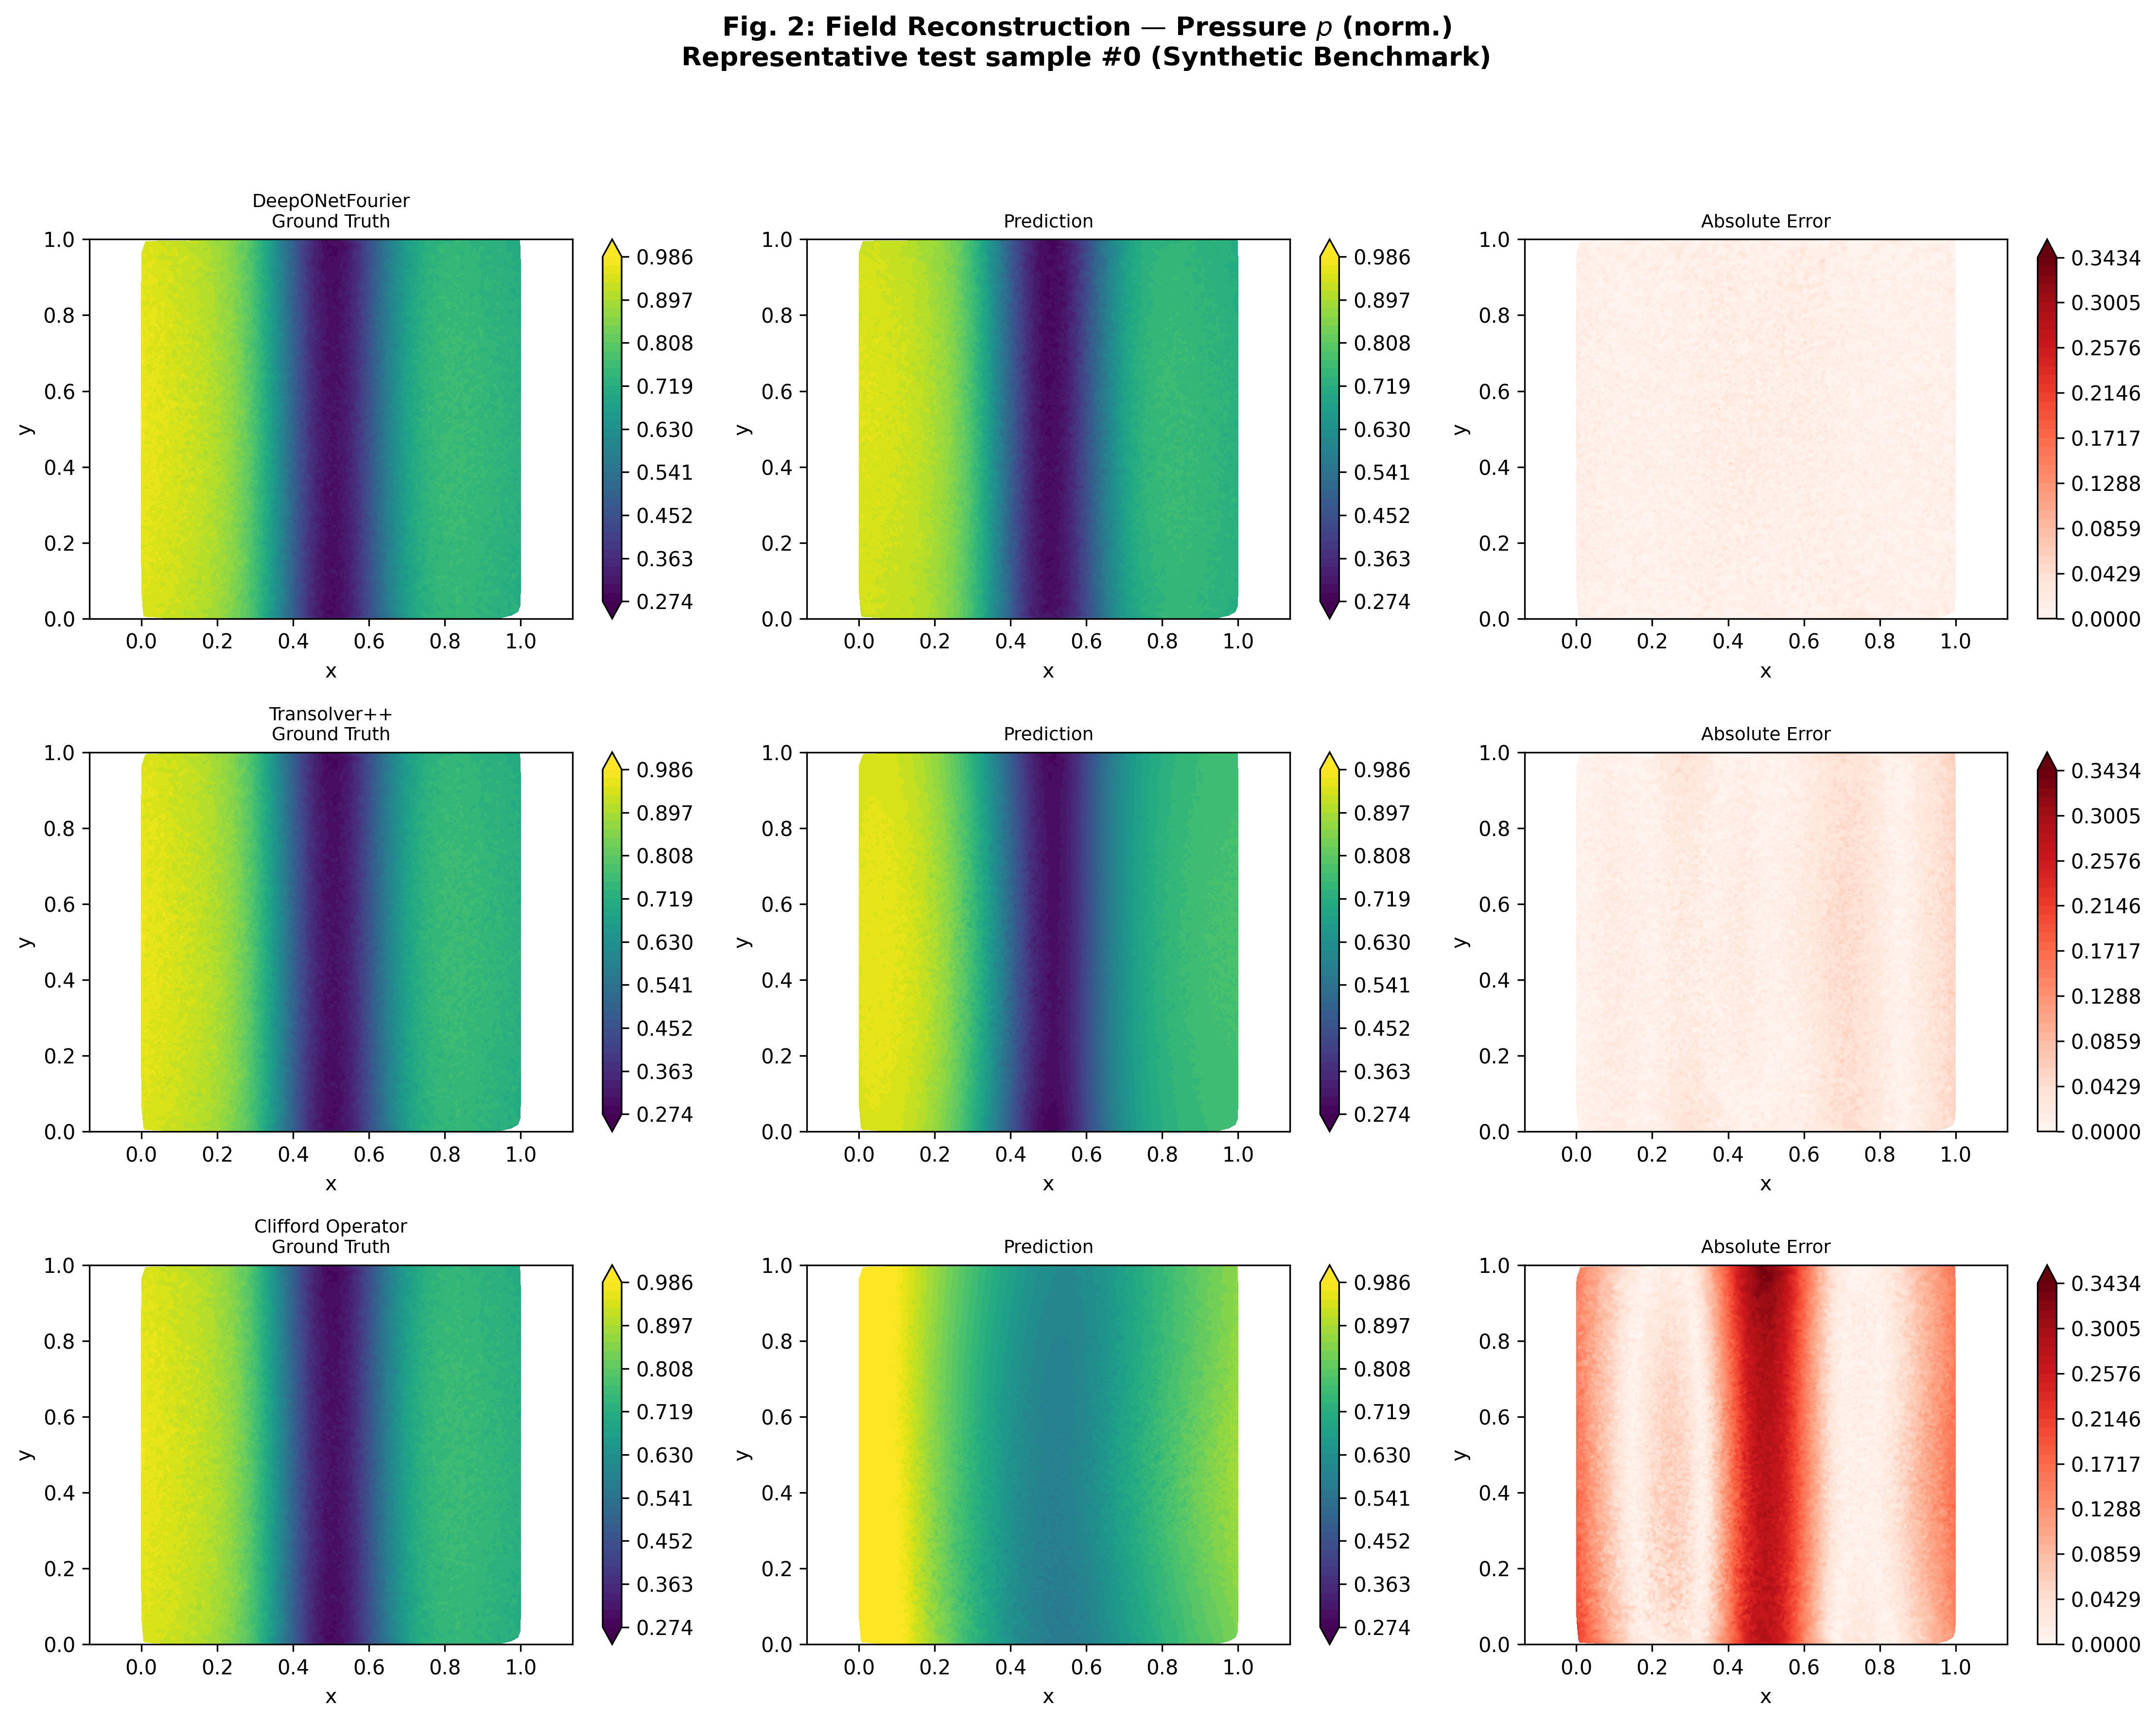
\includegraphics[width=\textwidth]{../../results/plots/paper_figures/fig_2_pressure_lossless.png}
\caption{\added{Normalized pressure reconstruction for held-out synthetic case~0. Rows show DeepONetFourier, Transolver++, and Clifford; columns show common-scale ground truth, common-scale prediction, and common-scale absolute error.}}
\label{fig:pressure_compare}
\end{figure*}

\begin{figure*}[htbp]
\centering
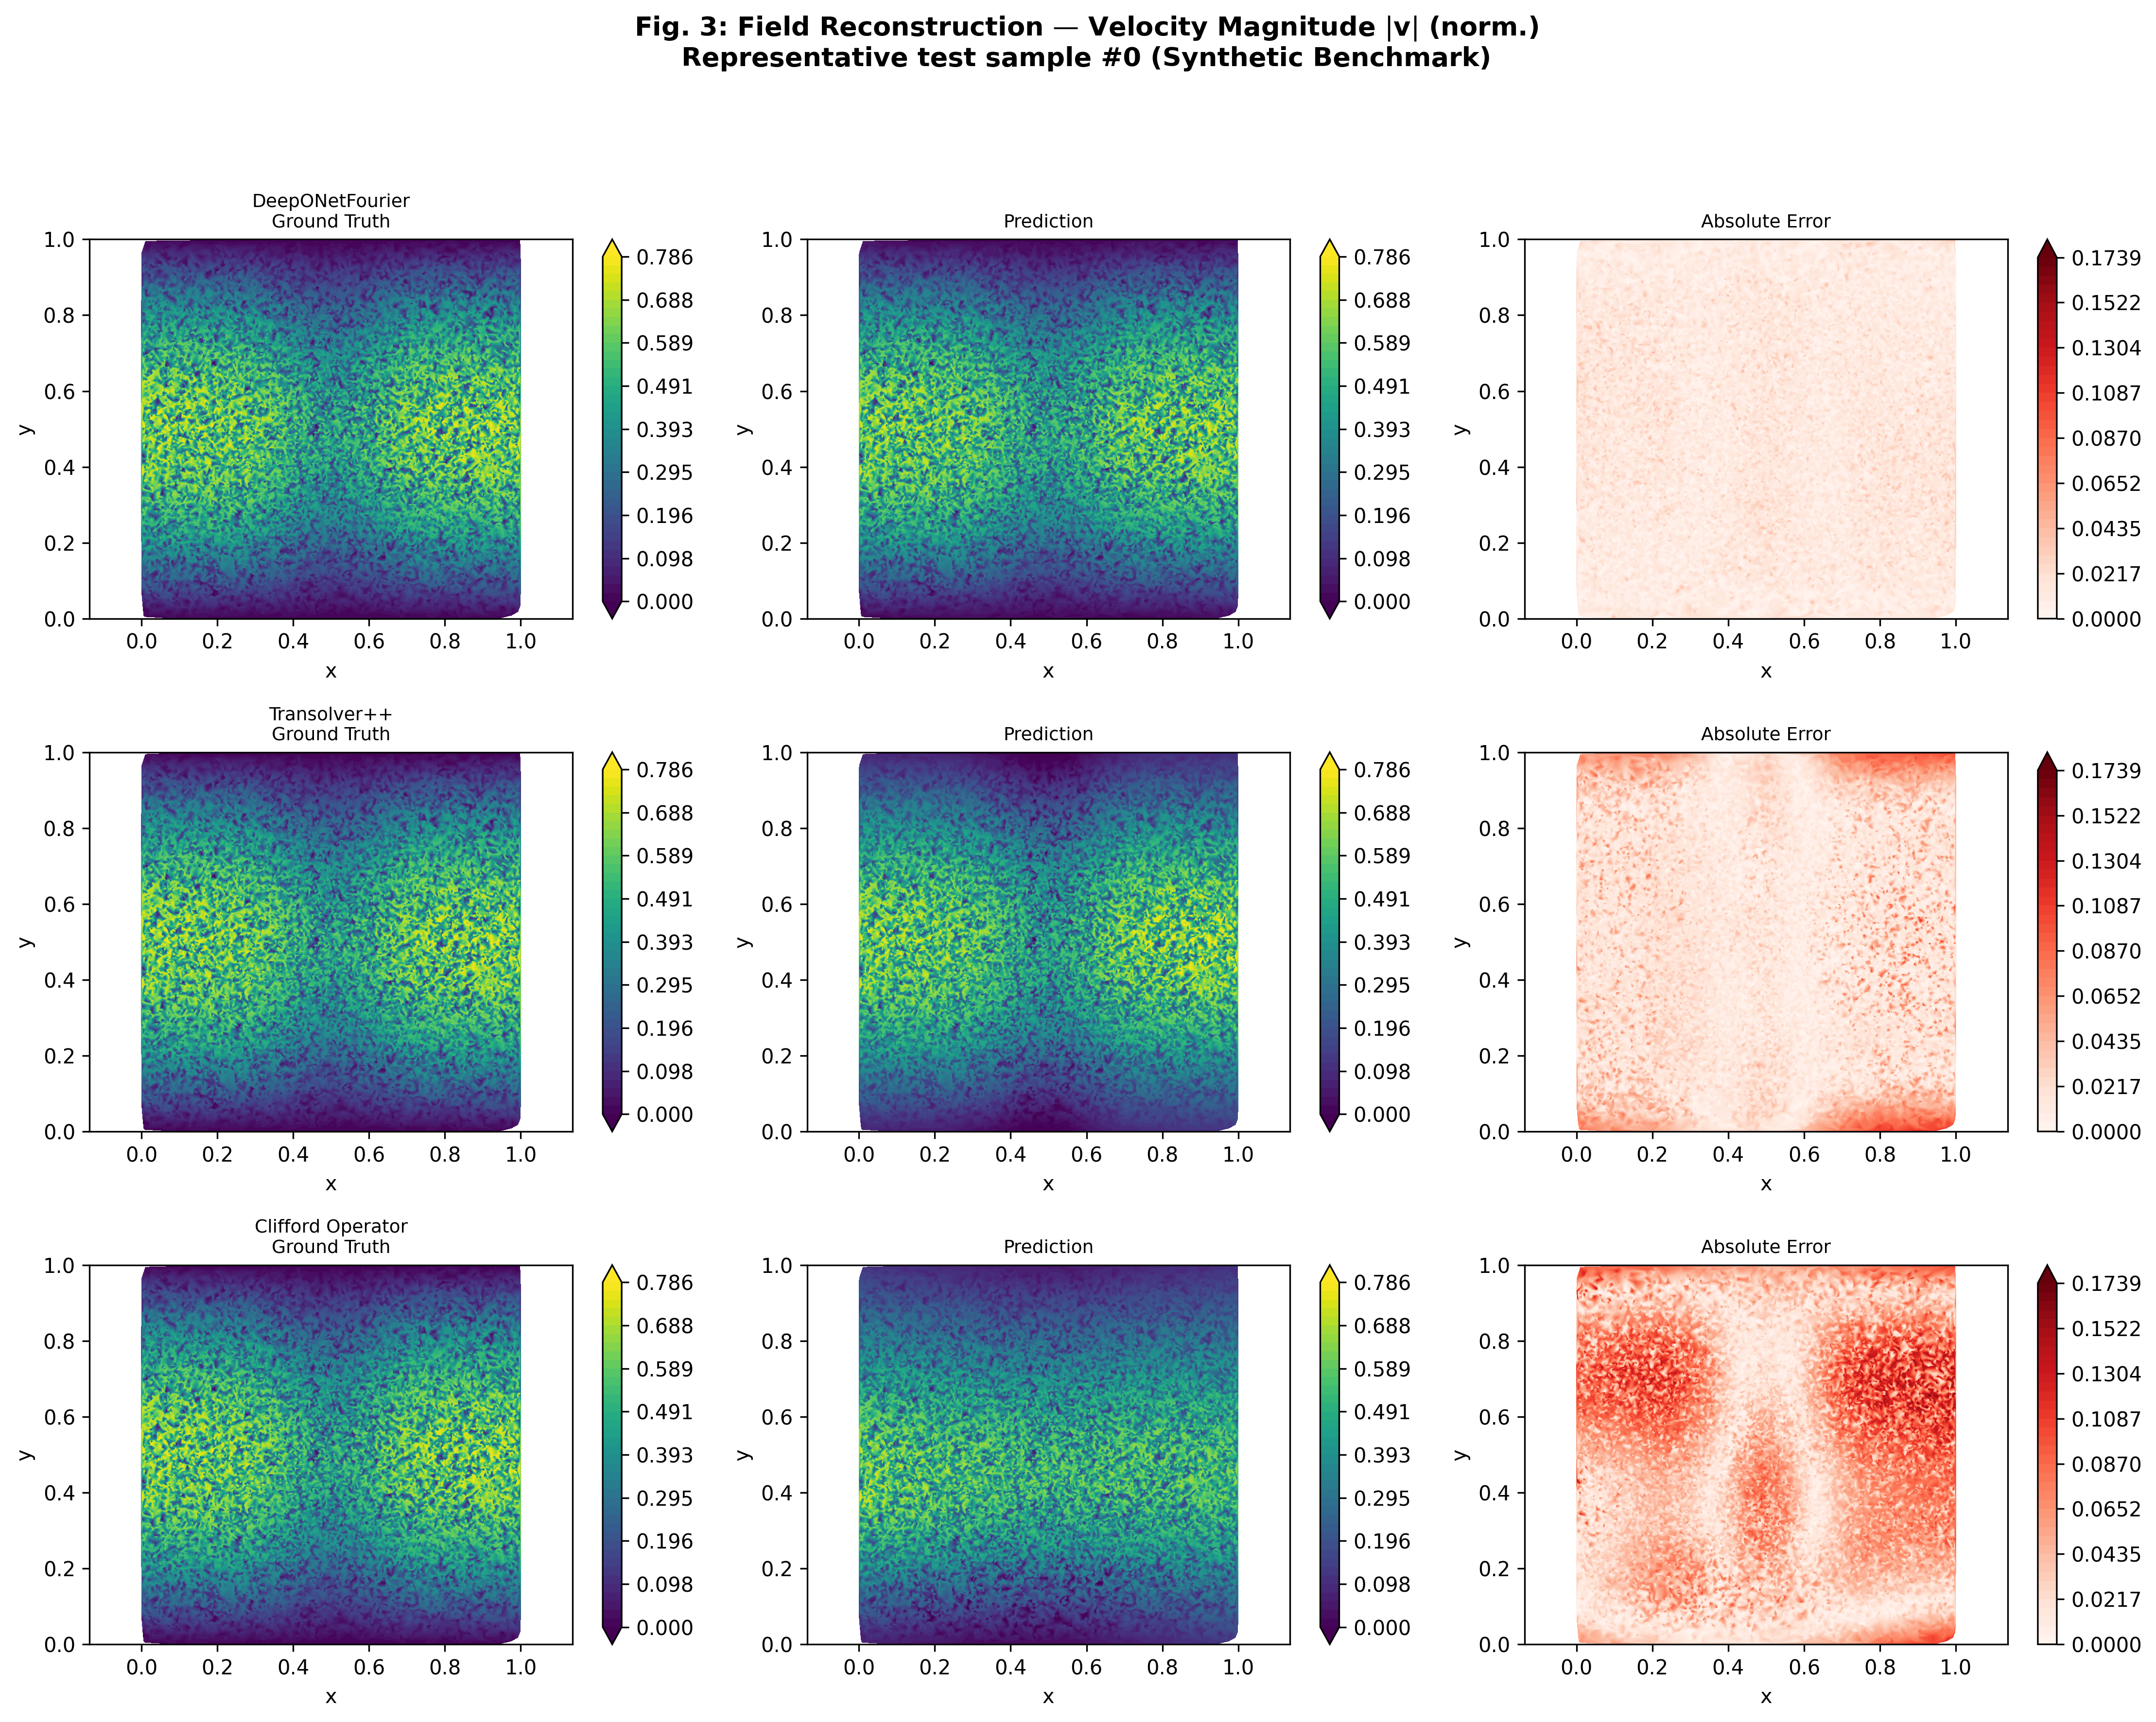
\includegraphics[width=\textwidth]{../../results/plots/paper_figures/fig_3_velocity_magnitude_lossless.png}
\caption{\added{Normalized velocity-magnitude reconstruction for held-out synthetic case~0, using the matched layout and scales described in Fig.~\ref{fig:pressure_compare}.}}
\label{fig:velocity_compare}
\end{figure*}

\begin{figure*}[htbp]
\centering
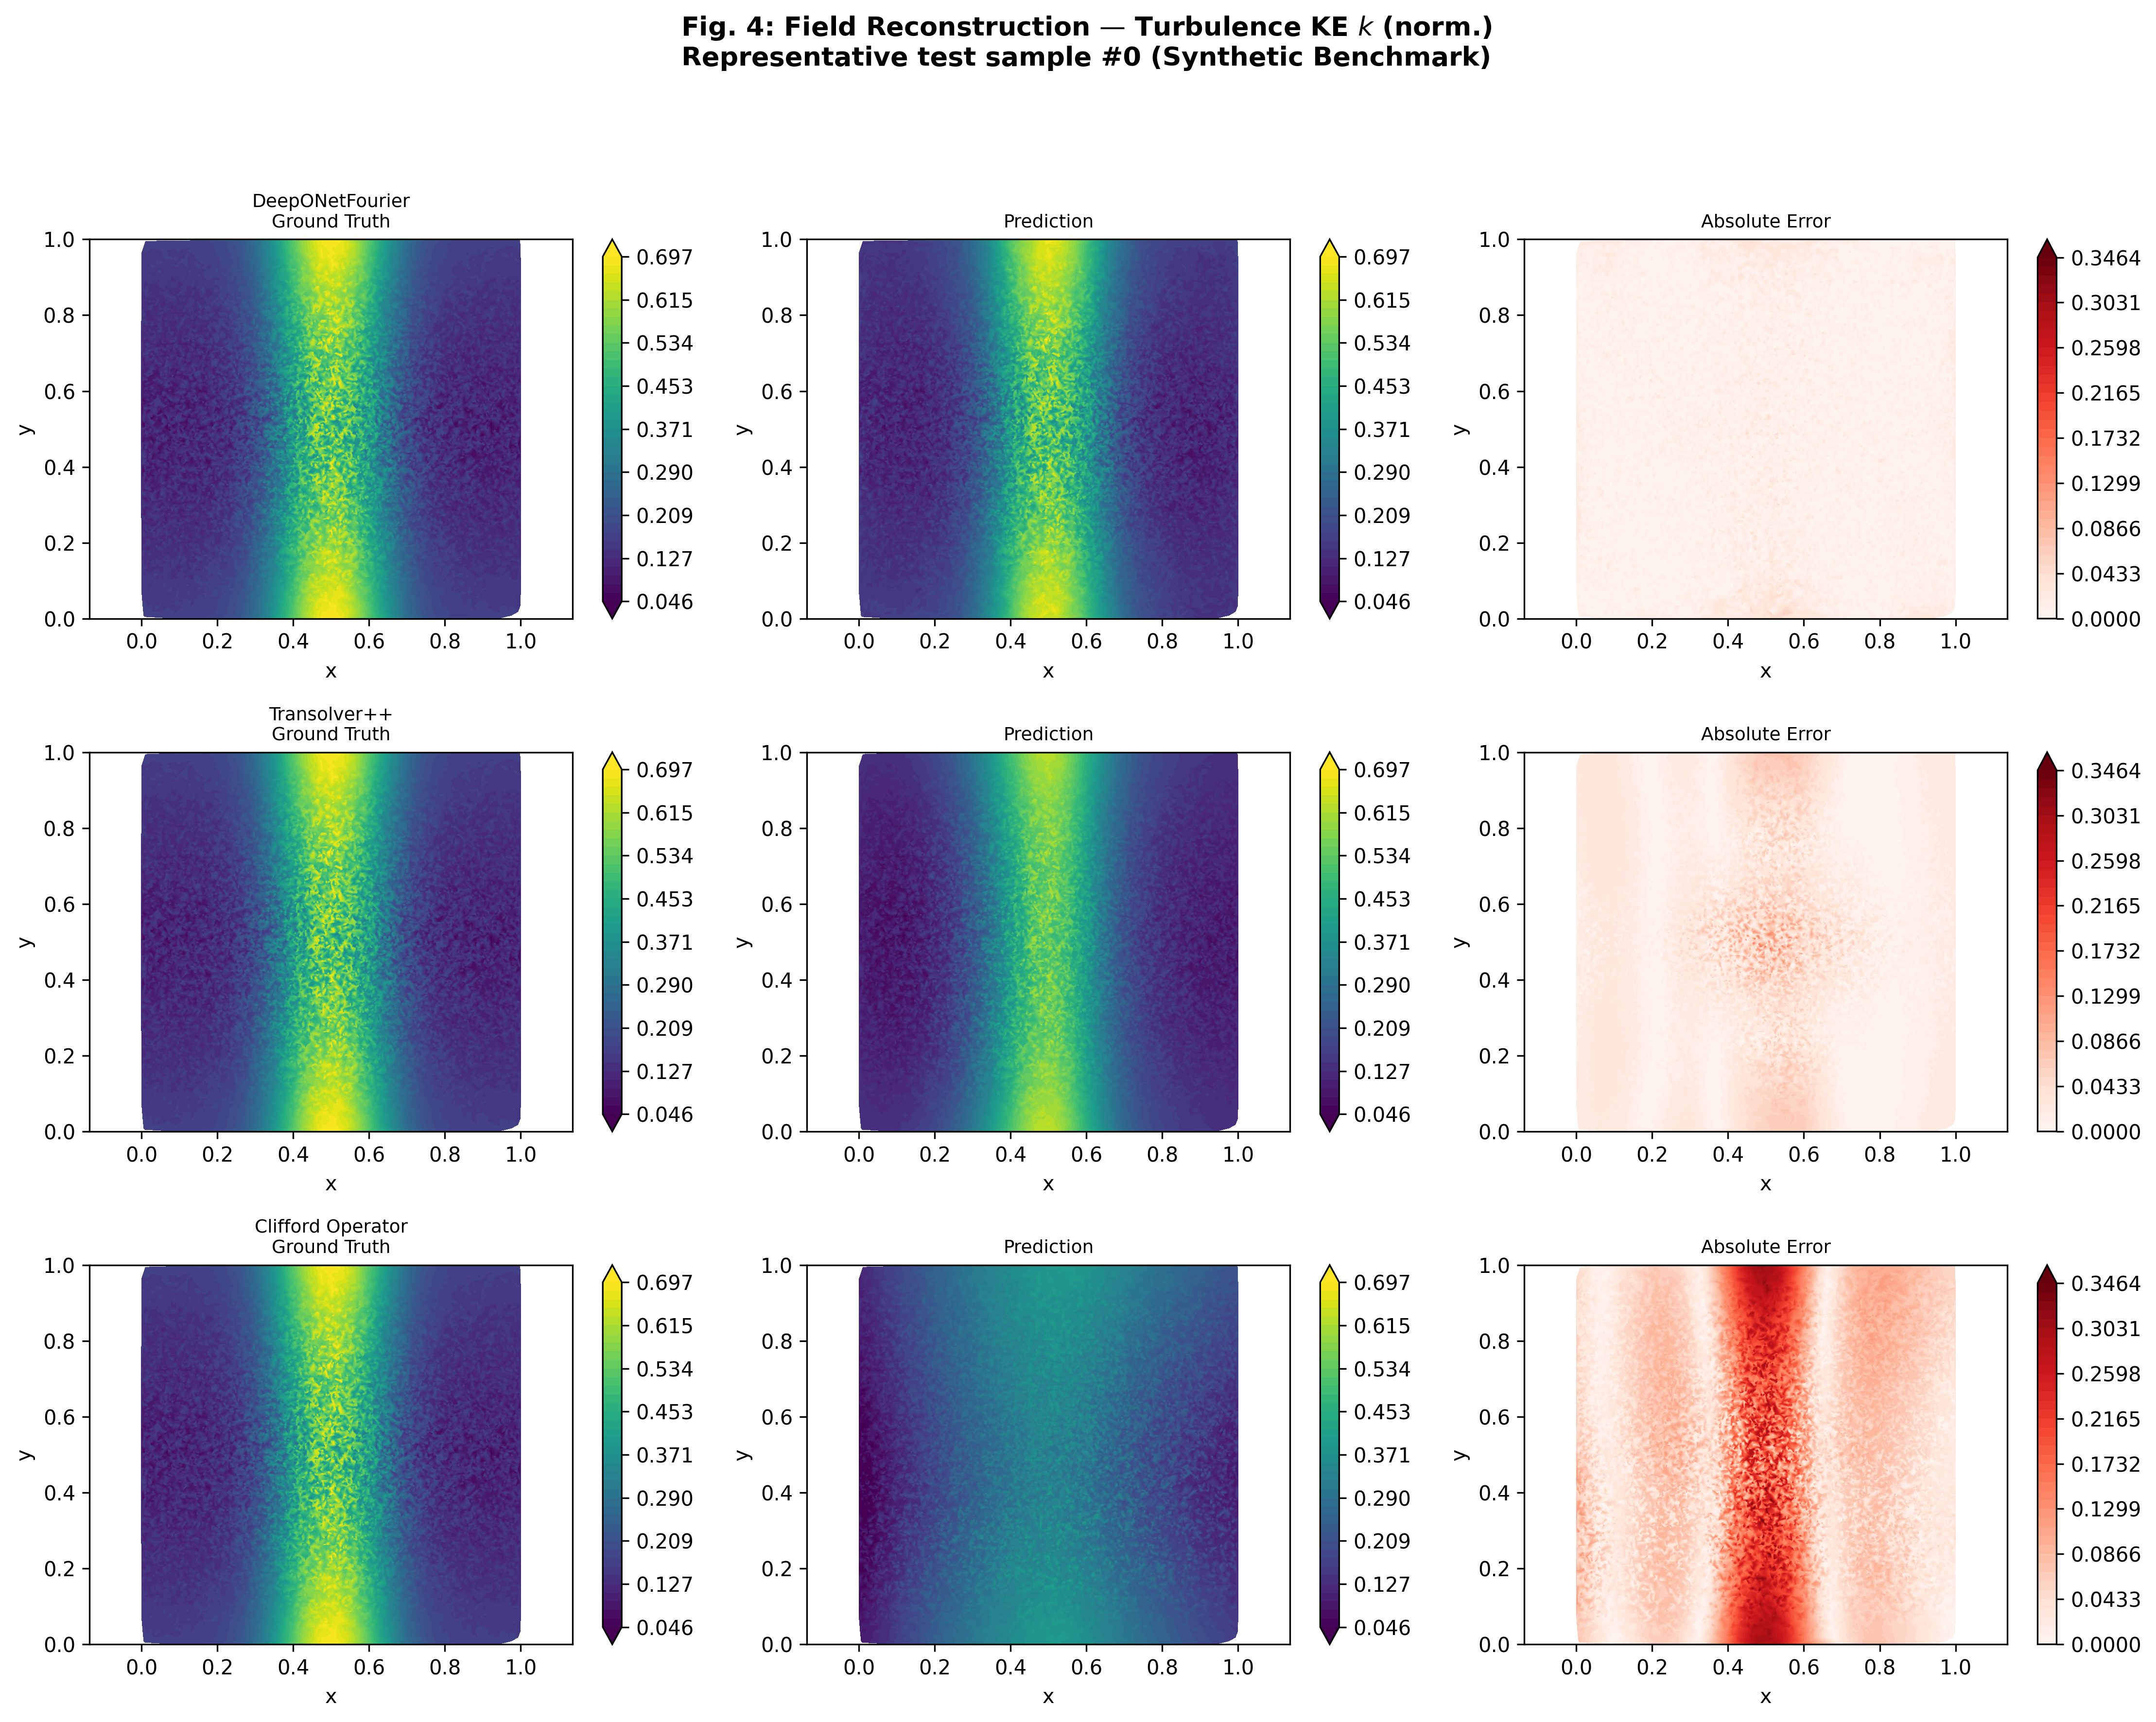
\includegraphics[width=\textwidth]{../../results/plots/paper_figures/fig_4_turbulence_k_lossless.png}
\caption{\added{Normalized turbulent-kinetic-energy reconstruction for held-out synthetic case~0, using the matched layout and scales described in Fig.~\ref{fig:pressure_compare}.}}
\label{fig:tke_compare}
\end{figure*}

\begin{figure*}[htbp]
\centering
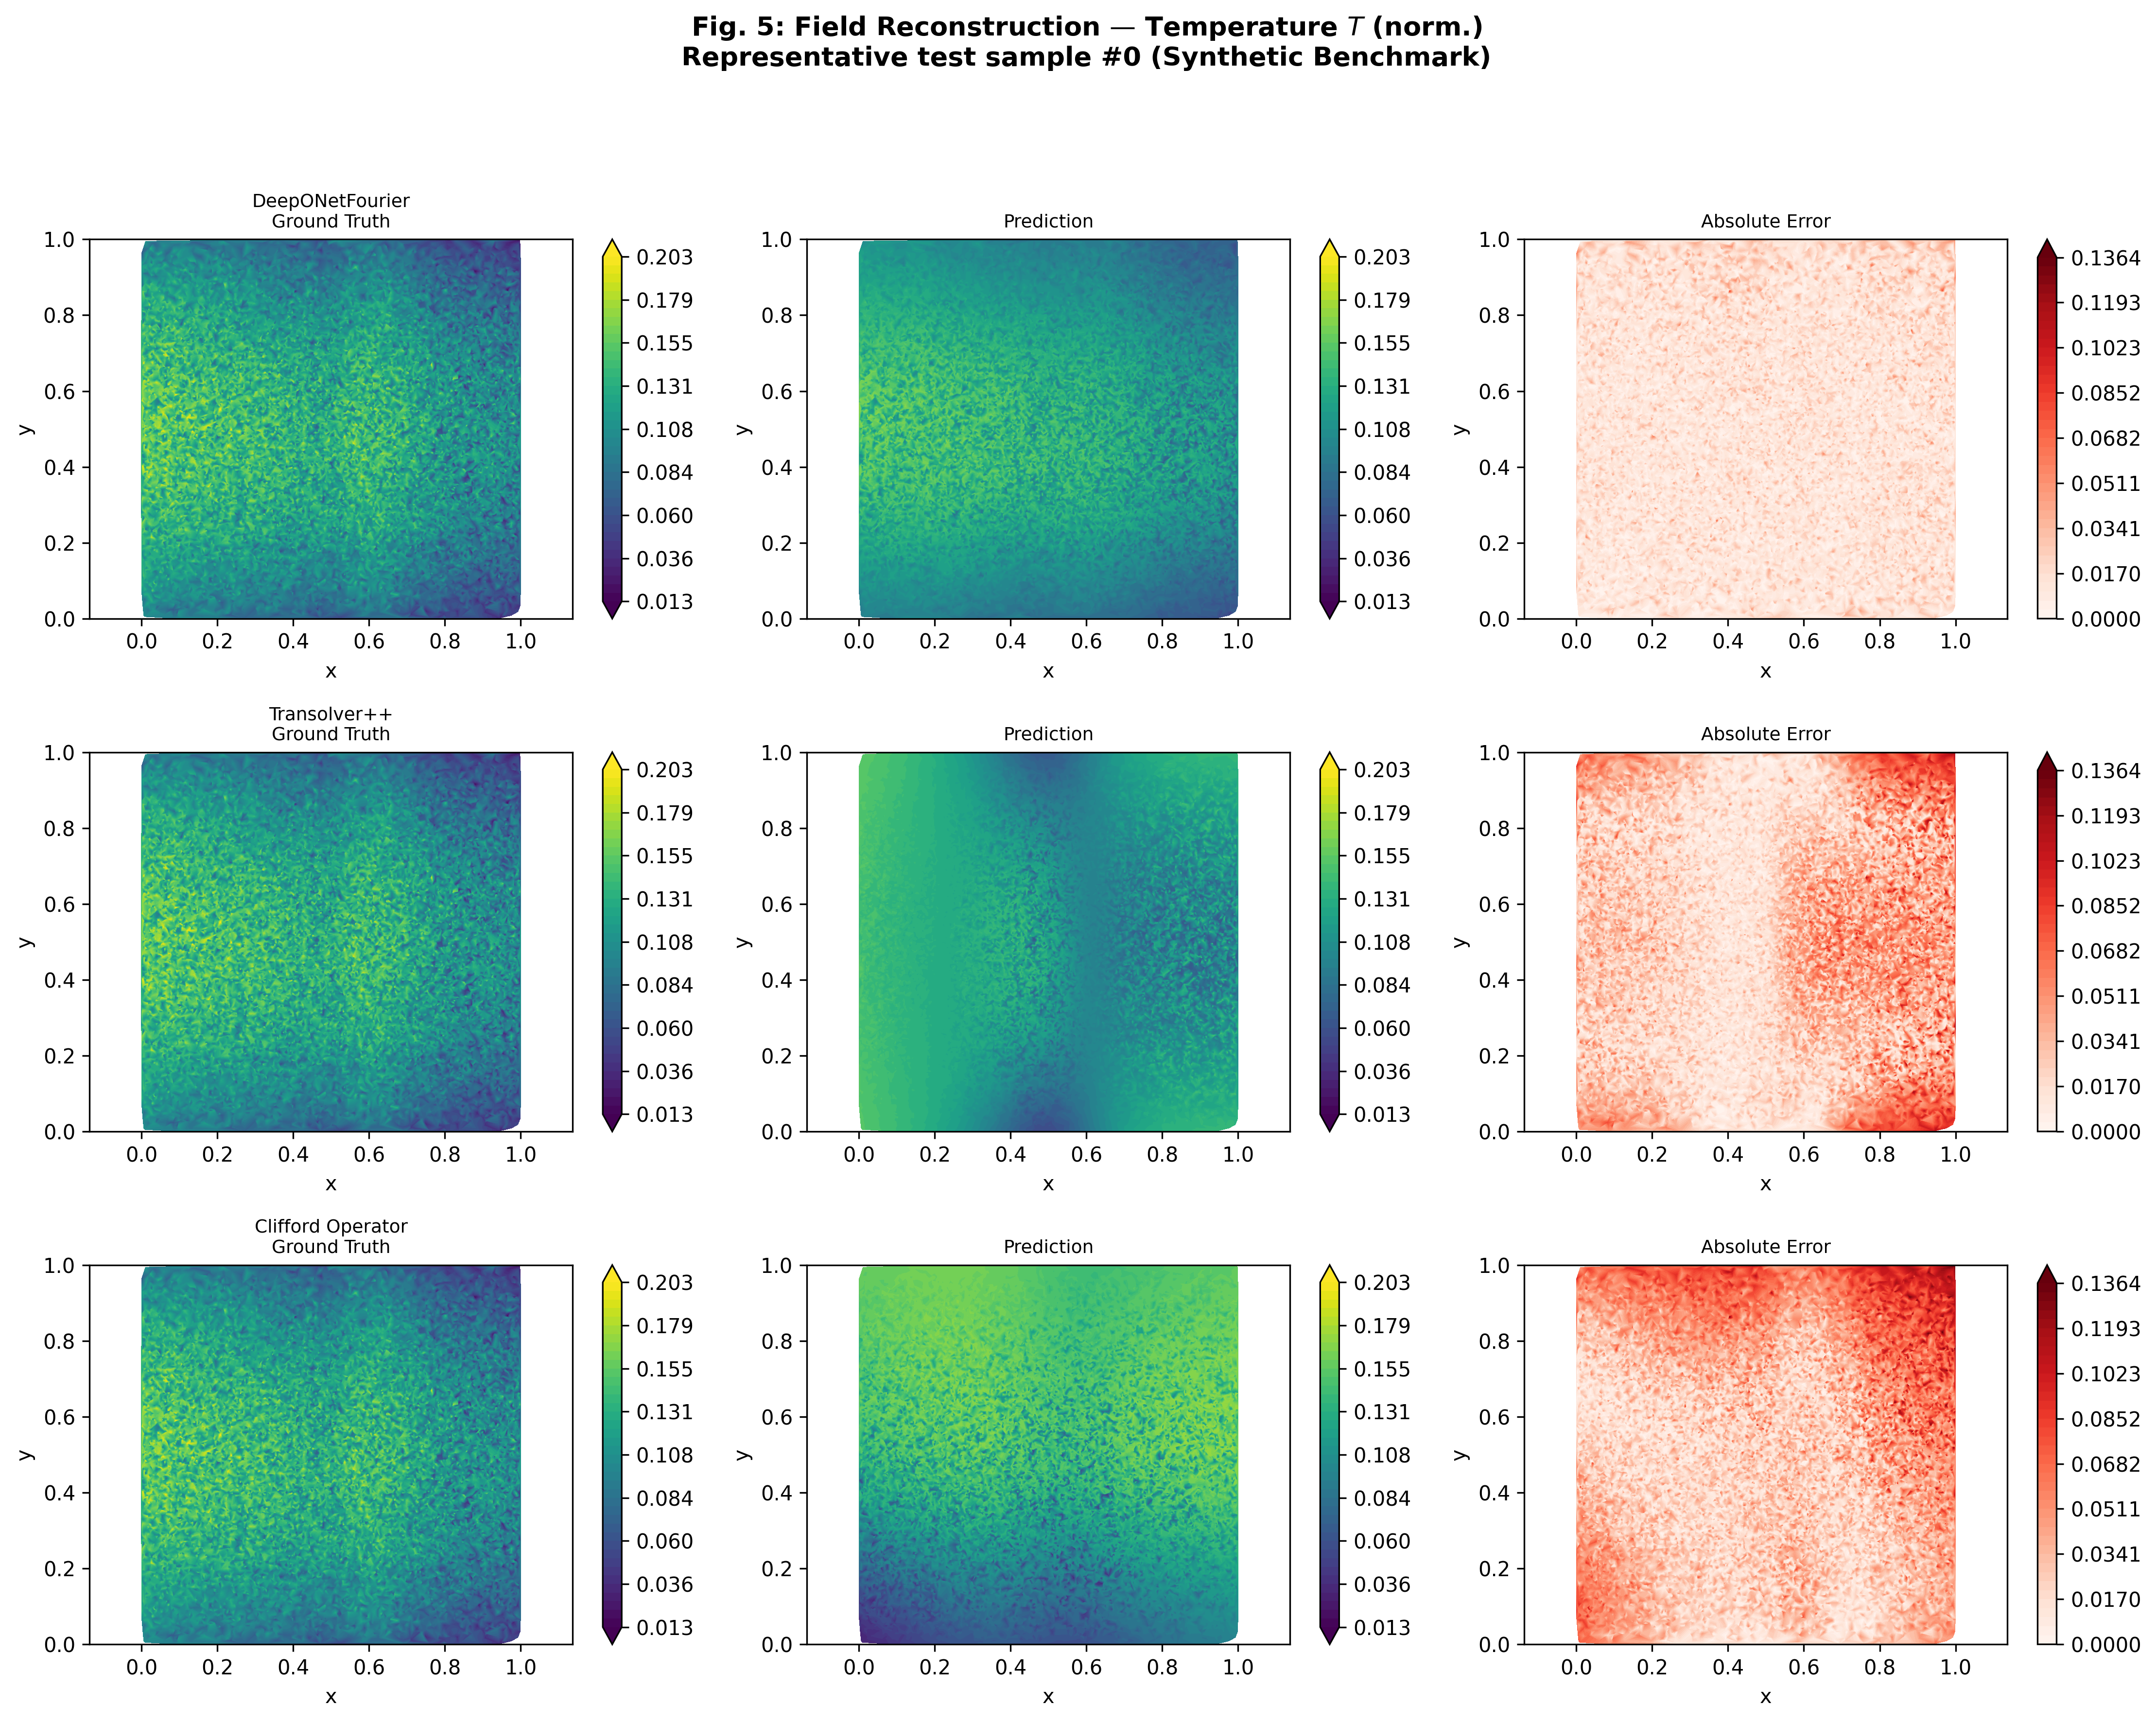
\includegraphics[width=\textwidth]{../../results/plots/paper_figures/fig_5_temperature_lossless.png}
\caption{\added{Normalized temperature reconstruction for held-out synthetic case~0, using the matched layout and scales described in Fig.~\ref{fig:pressure_compare}.}}
\label{fig:temperature_compare}
\end{figure*}

Table~\ref{tab:field_metrics} summarizes DeepONetFourier field accuracy on the 300-sample test set under the synthetic benchmark.

\begin{table}[htbp]
\caption{\added{DeepONetFourier Pooled Field Accuracy (All 300 Held-Out Synthetic Cases, Single Archived Checkpoint)}}
\label{tab:field_metrics}
\centering
\resizebox{\columnwidth}{!}{%
\begin{tabular}{lrrr}
\toprule
\textbf{Field} & \textbf{R$^2$} & \textbf{Rel.\,$L_2$} & \textbf{MAE (norm.)} \\
\midrule
Pressure & \added{0.9961} & \added{0.0158} & \added{0.00947} \\
Velocity magnitude & \added{0.9958} & \added{0.0348} & \added{0.01056} \\
Turbulence $k$ & \added{0.9951} & \added{0.0449} & \added{0.00666} \\
Temperature & \added{0.9962} & \added{0.0278} & \added{0.01221} \\
\bottomrule
\end{tabular}
}
\end{table}

\added{Here, pooled $R^2=1-\sum_i(y_i-\hat y_i)^2/\sum_i(y_i-\bar y)^2$, relative $L_2=\|\hat{\bm y}-\bm y\|_2/\|\bm y\|_2$, and MAE is computed after flattening all cases and nodes for each normalized field. Per-case $R^2$ means (population SD) were 0.9879 (0.0137), 0.9950 (0.0011), 0.9675 (0.0569), and 0.7355 (0.0126), respectively. Temperature's lower per-case $R^2$ reflects its small within-case spatial variance despite high pooled performance; reporting both scopes prevents metric-selection ambiguity.}

\subsection{Neural Operator Comparison}

\begin{table*}[htbp]
\caption{\added{Neural Operator Artifact Comparison (Synthetic Benchmark; Non-Identical Loss Settings)}}
\label{tab:benchmark}
\centering
\resizebox{\textwidth}{!}{%
\begin{tabular}{lccc}
\toprule
\textbf{Metric} & \textbf{DeepONet-F} & \textbf{Transolver} & \textbf{Clifford} \\
\midrule
Total parameters & 1,451,012 & \added{3,244,872} & \added{37,380} \\
Model-only forward pass (best observed, batch size 1) & $< 5$\,ms & $< 15$\,ms & $< 5$\,ms \\
End-to-end latency & $< 20$\,ms & $< 20$\,ms & $< 20$\,ms \\
Exact pooled test $R^2$ & 0.9951--0.9962 & \todo{multi-seed evaluation} & \todo{multi-seed evaluation} \\
Output shape & $[B,4,N]$ & $[B,4,N]$ & $[B,4,N]$ \\
Training objective & MSE + index proxies & MSE & MSE \\
Evaluated geometry & Fixed shared mesh & Fixed shared mesh & Fixed shared mesh \\
\bottomrule
\end{tabular}
}
\end{table*}

\textbf{Key observations under the present benchmark:}
\begin{itemize}
    \item \textbf{DeepONetFourier} reconstructs the four synthetic fields with pooled $R^2=0.9951$--0.9962 on one fixed-mesh checkpoint.  \added{Its different objective prevents attributing any comparative advantage to architecture alone.}
    \item \textbf{Transolver++} supplies global token attention and has 3.245M parameters. 
    \item \textbf{Clifford Operator} is compact at 37,380 parameters.  \added{Those properties require dedicated learning-curve and rotation-consistency experiments.}
\end{itemize}

\subsection{LOCA Indicator Classification Performance}

Fig.~\ref{fig:locac_perf} shows the LOCA indicator detection performance panel, and Table~\ref{tab:locac_metrics} summarizes classifier metrics. As discussed in Section~\ref{sec:pipeline}, the classifier output is substantially driven by the input break-size parameter via $\eta_\text{eff}$, so these results should be read as an indicator-translation demonstration rather than as end-to-end digital twin validation.

\begin{figure}[htbp]
\centering
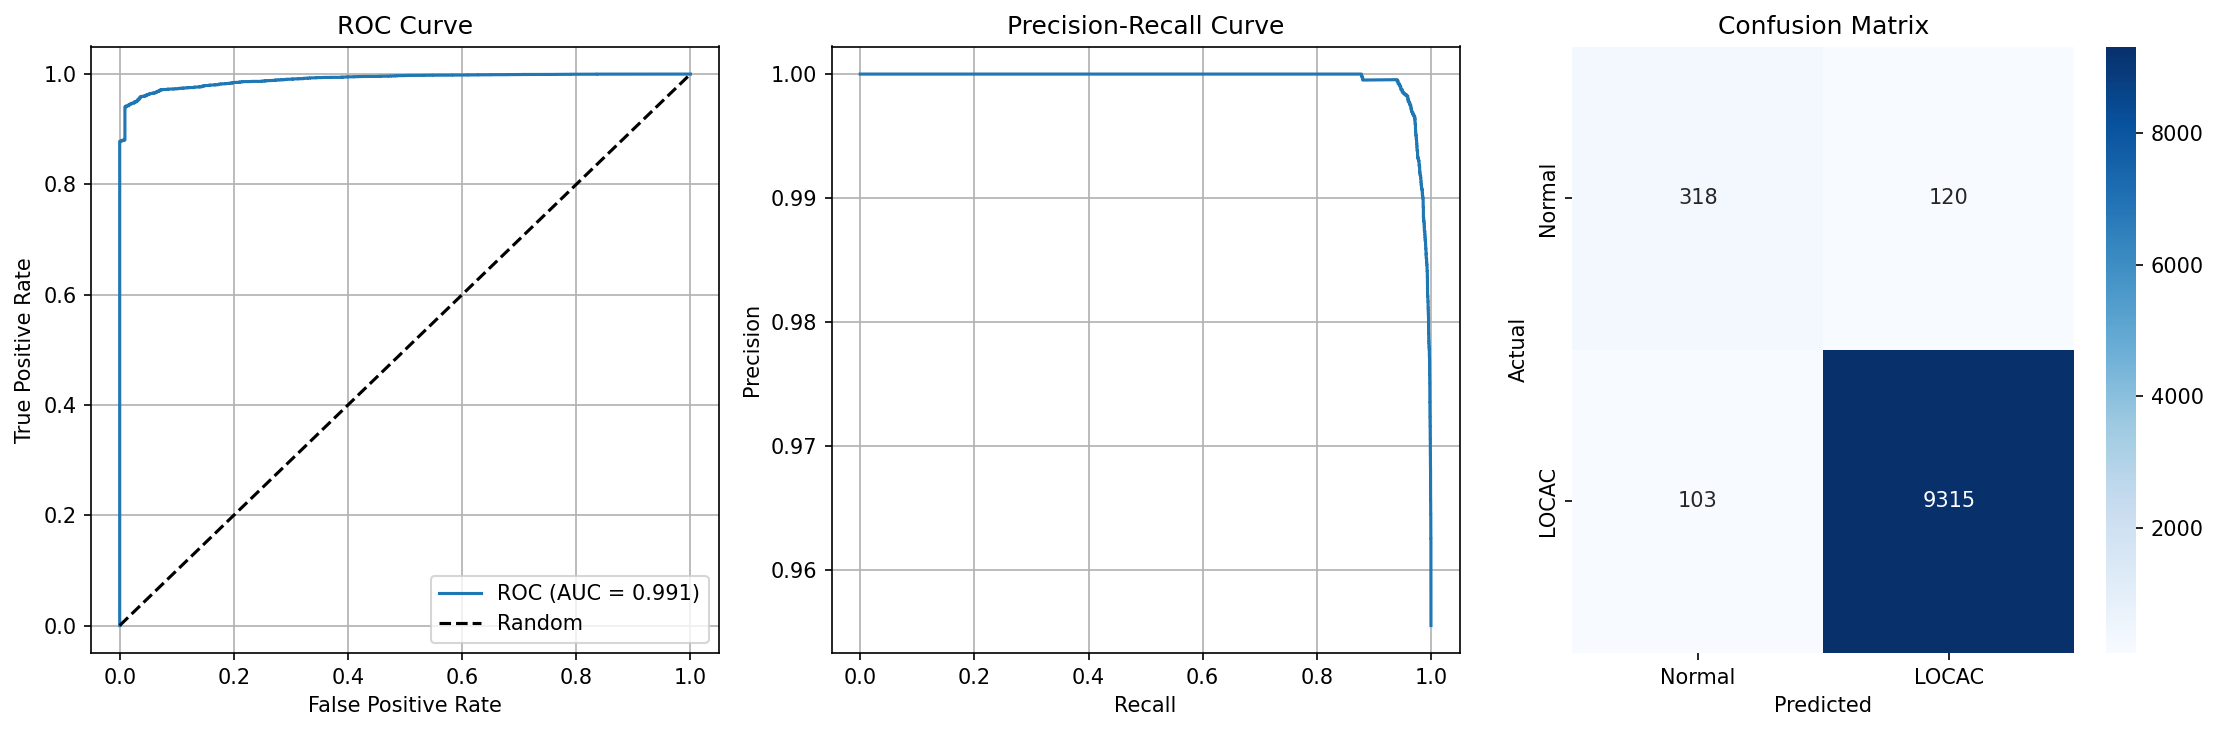
\includegraphics[width=\columnwidth]{../../results/plots/locac_detection_performance.png}
\caption{\added{Classifier ROC curve (AUC 0.990554), precision--recall curve, and confusion matrix for one seed-42 split of PCTRAN-simulated NPPAD rows plus synthetic transition augmentation. This is classifier-level evidence, not independent end-to-end digital-twin validation.}}
\label{fig:locac_perf}
\end{figure}

\begin{table}[htbp]
\caption{\added{LOCA Indicator Classifier Performance (NPPAD-Simulated + Synthetic Transition Data, One Seed-42 Split)}}
\label{tab:locac_metrics}
\centering
\begin{tabular}{ll}
\toprule
\textbf{Metric} & \textbf{Score} \\
\midrule
Accuracy & \added{0.977374} \\
Precision & \added{0.987281} \\
Recall (Sensitivity) & \added{0.989063} \\
F1 Score & \added{0.988172} \\
ROC-AUC & \added{0.990554} \\
\bottomrule
\end{tabular}
\end{table}

\begin{table}[htbp]
\caption{\added{Five-Seed Translation-Path Ablation (mean $\pm$ population SD). The direct severity term is removed in the second column, but label-conditioned break size remains an operator input.}}
\label{tab:translation_ablation}
\centering
\begin{tabular}{lcc}
\toprule
\textbf{Metric} & \textbf{80/20 Blend} & \textbf{Direct Term Removed} \\
\midrule
ROC-AUC & 0.999997 $\pm$ 0.000003 & 0.999977 $\pm$ 0.000046 \\
Recall & 1.000000 $\pm$ 0.000000 & 1.000000 $\pm$ 0.000000 \\
F1 & 0.999956 $\pm$ 0.000041 & 0.999989 $\pm$ 0.000022 \\
Accuracy & 0.999912 $\pm$ 0.000082 & 0.999978 $\pm$ 0.000044 \\
\bottomrule
\end{tabular}
\end{table}

 \added{The archived classifier metrics do not retain a break-size-stratified error analysis, and no reliability diagram, Brier score, or expected calibration error was computed. Table~\ref{tab:probability} therefore reports only the monotonic response of the mapped classifier score in the synthetic translation demonstration.} \todo{Evaluate the classifier across at least five independent group-aware splits and report threshold-dependent POD/false-alarm curves plus calibration metrics with confidence intervals.}

\begin{table}[htbp]
\caption{\added{Mapped LOCA-Score Response vs. Prescribed Break Size (Synthetic Translation Demonstration; Not a Calibration Result)}}
\label{tab:probability}
\centering
\begin{tabular}{cc}
\toprule
\textbf{Break Size (\%)} & \textbf{Mapped LOCA Score} \\
\midrule
0 (Normal) & $\approx 0.10$ \\
2 & $\approx 0.13$ \\
4 & $\approx 0.40$ \\
5 (threshold) & $\approx 0.56$ \\
7 & $\approx 0.74$ \\
10 (severe) & $\approx 0.91$ \\
\bottomrule
\end{tabular}
\end{table}

\subsection{Inference Speed}

End-to-end pipeline latency is reported below 20\,ms under the present RTX~4060 implementation, with the timing boundary comprising neural-operator inference, feature translation, and classification for one case. Dividing the \added{conservative assumed lower-bound} Fluent duration of 3,600\,s by 0.020\,s gives \textbf{${\sim}180{,}000\times$}.  \added{It is an illustrative reference ratio: the source artifact does not contain a Fluent run timed on matched hardware, and preprocessing/data-transfer boundaries are not matched.} \todo{Archive warm-up policy, synchronization method, repetitions, latency distribution, hardware/software versions, and a measured Fluent comparator before reporting a benchmark speedup.}

%═══════════════════════════════════════════════════════════════════════════════
\section{Discussion}
\label{sec:discussion}
%═══════════════════════════════════════════════════════════════════════════════

\subsection{Methodological Contributions}

This work makes three primary methodological contributions. First, it demonstrates that three distinct neural-operator paradigms---enhanced branch--trunk decomposition, mesh-token attention, and geometric-algebra encoding---can share one surrogate-to-indicator pipeline. Second, it establishes exact synthetic-test metrics for the archived DeepONetFourier checkpoint and a dataset-matched unmodified DeepONet baseline while documenting the non-identical objectives.  \added{Code inspection instead identifies two index-space proxy terms, preventing a conservation claim and motivating a geometry-aware retraining experiment.} Third, the work exposes rather than hides the current validation boundary: analytic fields, PCTRAN-simulated classifier data, label-conditioned translation, single-run operator results, and an assumed CFD time reference.

\subsection{Architectural Trade-Off Analysis}

The three architectures address different deployment priorities and the following observations are framed as \emph{preliminary inductive-bias findings} under non-identical optimization settings:

\textbf{DeepONetFourier} achieved the only fully recomputed 300-case test metrics in this revision and has 54.1\% fewer parameters than the retrained DeepONet baseline. Fourier encoding is an explicit high-frequency representation mechanism; the incremental effects of that encoding, adaptive activation, and the two proxy terms have not been isolated under matched retraining.

\textbf{Transolver++} provides global interactions over $M=64$ tokens, with $\mathcal{O}(M^2)$ token-attention complexity, and is the largest studied model at 3.245M parameters.  \added{Because all training and evaluation use the same mesh, transfer across topology is a hypothesis rather than a result.}

\textbf{Clifford Operator} is the most compact studied model at 37,380 parameters. Its internal Cl(3,0) operations preserve a useful grade structure, but the dense $256\to4$ decoder mixes grades.  \added{Learning-curve and rotation-consistency experiments are required before either advantage can be asserted.}

\subsection{Surrogate-Monitoring Utility and Limits of Current Validation}

The current results represent upper-bound methodological performance under controlled, physics-consistent synthetic conditions. Several important caveats apply:

The synthetic mock generator produces fields that are physics-\emph{consistent} but not physics-\emph{exact}: they incorporate qualitative pipe-flow structures but are generated analytically rather than by a validated flow solver. The pooled $R^2=0.9951$--0.9962 values therefore quantify interpolation on that synthetic generator's distribution, not accuracy relative to Fluent CFD, experiments, or plant transients.

The blended severity model ($\eta_\text{eff}=0.8\eta_\text{input}+0.2\eta_\text{CFD}$) means the main LOCA score is substantially driven by prescribed break size. The available five-seed ablation removes the explicit translator term, but its break-size input is sampled conditionally on the class.  \added{A label-independent evaluation remains necessary to quantify whether reconstructed fields add detection information.}

\subsection{Path to Full-Fidelity Validation}

The natural next step is ANSYS Fluent validation over the parameter space already established in this paper: low, medium, and high break severities ($b \approx 2\%, 5\%, 10\%$), multiple inlet velocities ($v \in \{4.0, 5.0, 6.0\}$\,m/s), the same AP1000 cold-leg geometry, and the same field metrics reported here ($R^2$, relative $L_2$, MAE). Because the Fluent production pathway is already described in Stage~1 and implemented in the codebase, this is a credible and concrete near-term extension---and full-fidelity validation is necessary before any deployment claim can be made.

\subsection{Limitations and Future Work}
\label{sec:limitations}

\textbf{Missing baselines}:  \added{A dataset-matched unmodified DeepONet result is now included, but plain MLP and FNO baselines remain absent. A component ablation is also required to isolate Fourier features, adaptive activations, and each proxy term.}

\textbf{Run-to-run stability}: Operator results and the primary classifier artifact are single-run. Only the constrained translation-path ablation has five seeds. \todo{Complete the predeclared five-seed operator and classifier protocols and report mean $\pm$ sample SD with run manifests.}

\textbf{Non-identical optimization}: DeepONetFourier uses a doubled value-fidelity term plus index-gradient and velocity-variation proxies, whereas the other operators use MSE only. A controlled comparison requires matched objectives and tuning budgets; present cross-architecture figures are qualitative artifact inspections, not a ranking.

\textbf{Steady-state assumption}: LOCA events are transient, and the present results address only steady-state field reconstruction.  \added{No enabled configuration, checkpoint, or transient result was found for that module; a temporal operator is therefore future work only.} \todo{Construct a transient CFD/NPPAD-aligned split, train the temporal model, and report sequence-level detection delay, POD, false alarms, and distribution-shift tests.}

\textbf{Uncertainty quantification}: The evaluated pipeline produces point predictions and classifier scores only.  \added{Diffusion is disabled by default; no trained diffusion checkpoint, held-out sampling protocol, coverage result, or decision-level propagation artifact was found. DDPM-based turbulence sampling is unevaluated future work, and a classifier score is not predictive uncertainty.} \todo{Train on held-out cases; report nominal versus empirical coverage, interval width, proper scores, and calibration; then propagate samples through feature translation and classification end to end.}

\textbf{Detection-threshold and false-alarm analysis}: The classifier currently reports performance at a single decision threshold (0.5) via aggregate metrics (ROC-AUC, recall, F1). A reliability-oriented treatment should additionally report the detection-threshold/false-alarm-rate trade-off explicitly (e.g., an operating-point analysis tied to an acceptable false-alarm budget for operator-facing screening), since false negatives and false positives carry very different consequences in a LOCA-screening context.

\textbf{AI-model failure modes}: This study does not analyze distribution shift between analytic synthetic fields and Fluent/experimental data, robustness to noise or simulator shift in the PCTRAN-derived features, or behavior outside $v\in[4.0,6.0]$\,m/s, $b\in[0,10]\%$, and $T\in[290,320]^\circ$C. Such evidence is central to a reliability argument \cite{nrc7294,trilateral2024}.

\textbf{Multi-fidelity learning}: A residual multi-fidelity module combining coarse-RANS and fine-LES predictions ($u_\text{final} = u_\text{base} + u_\text{residual}$) is a planned extension; not evaluated in the present results.

\textbf{Wall shear stress}: A post-processing module for $\tau_w = \mu\,\partial u/\partial y$ with corrosion-risk assessment is a planned extension for pipe-integrity monitoring; not evaluated in the present results.

%═══════════════════════════════════════════════════════════════════════════════
\section{Conclusion}
\label{sec:conclusion}
%═══════════════════════════════════════════════════════════════════════════════

This paper has presented a proof-of-concept, multi-architecture neural operator digital twin for Cold-Leg LOCA screening in the AP1000 PWR, comparing three neural-operator paradigms and coupling the archived DeepONetFourier surrogate to a downstream classification pipeline. The principal findings, all obtained under the synthetic, physics-consistent benchmark described in Section~\ref{sec:problem}, are as follows:

\begin{itemize}
    \item \textbf{DeepONetFourier} has 1,451,012 parameters, 54.1\% fewer than the 3,162,116-parameter retrained DeepONet baseline. Its archived checkpoint attains pooled test $R^2=0.9951$--0.9962 across the four synthetic fields.  \added{they are explicitly limited to index-space regularization.}
    \item \textbf{Transolver++} has 3,244,872 parameters and provides global attention over 64 mesh tokens.  \added{they are not retained as findings.}
    \item \textbf{Clifford Operator} has 37,380 parameters (approximately $38.8\times$ fewer than DeepONetFourier).  \added{rotation-aware decoding remains an experiment.}
    \item The single-split classifier artifact reaches ROC-AUC 0.990554, recall 0.989063, and F1 0.988172 on PCTRAN-simulated NPPAD rows plus synthetic transition augmentation. The five-seed translation-path ablation remains label-conditioned, so neither result establishes independent LOCA detection from predicted fields.
    \item End-to-end latency is reported below 20\,ms. The resulting $\sim$180,000$\times$ ratio uses an assumed conservative 3,600\,s Fluent lower bound and is not a matched CFD timing benchmark. 
\end{itemize}

Collectively, these results demonstrate methodological feasibility rather than validated screening capability. Full-fidelity CFD/experimental validation, geometry-aware physical derivatives, label-independent detection, matched-loss multi-seed evaluation, calibrated uncertainty, and a reliability safety case are prerequisites for any safety-relevant claim. The shared configuration interface makes those experiments tractable, but software integration alone is not evidence of operational readiness.

%─── Data Availability ────────────────────────────────────────────────────────
\section*{Data Availability Statement}
\added{Project source code, including the synthetic-data generator, is publicly available at \url{https://github.com/Punyansh26/Digital-Twin-for-NPP-Cold-Leg-LOCAC-detection}. The exact local split, checkpoints, metric JSON files, and revised figures used for this manuscript have not yet been deposited in a versioned archive and are available from the corresponding author upon reasonable request. NPPAD was created by its original authors with PCTRAN and is available from the publication and project repository cited in \cite{qi2022nppad}; it should be obtained from that source under its stated license rather than treated as original plant data collected by the present authors.} \todo{Before submission, deposit the exact data split, checkpoints, run manifests, metric JSON files, and figure-generation code in a persistent tagged repository/DOI archive and cite the release identifier.}

%─── Acknowledgment ───────────────────────────────────────────────────────────
\section*{Acknowledgment}
The authors acknowledge Qi \emph{et al.}~\cite{qi2022nppad} for the open PCTRAN-simulated NPPAD time-series dataset used in the classifier study.  The physics-consistent synthetic field generator used for neural-operator training and evaluation was developed as part of this project. Computational resources for the archived training runs included an NVIDIA RTX~4060 GPU.

%─── References ───────────────────────────────────────────────────────────────
\begin{thebibliography}{00}

\bibitem{lu2021deeponet}
L. Lu, P. Jin, G. Pang, Z. Zhang, and G. E. Karniadakis,
``Learning nonlinear operators via DeepONet based on the universal approximation theorem of operators,''
\textit{Nature Machine Intelligence}, vol.~3, pp.~218--229, 2021.

\bibitem{chen1995}
T. Chen and H. Chen,
``Universal approximation to nonlinear operators by neural networks with arbitrary activation functions and its application to dynamical systems,''
\textit{IEEE Trans.\ Neural Networks}, vol.~6, no.~4, pp.~911--917, 1995.

\bibitem{lu2022comprehensive}
L. Lu, X. Meng, S. Cai, Z. Mao, S. Goswami, Z. Zhang, and G. E. Karniadakis,
``A comprehensive and fair comparison of two neural operators (with practical extensions) based on fair data,''
\textit{Comput.\ Methods Appl.\ Mech.\ Engrg.}, vol.~393, p.~114778, 2022.

\bibitem{li2021fno}
Z. Li, N. Kovachki, K. Azizzadenesheli, B. Liu, K. Bhattacharya, A. Stuart, and A. Anandkumar,
``Fourier neural operator for parametric partial differential equations,''
in \textit{Proc.\ ICLR}, 2021.

\bibitem{wu2024transolver}
H. Wu, H. Luo, H. Wang, J. Wang, and M.~Long,
``Transolver: A fast transformer solver for PDEs on general geometries,''
in \textit{Proc.\ ICML}, 2024.

\bibitem{brandstetter2023clifford}
J. Brandstetter, R. Berg, M. Welling, and J. K. Gupta,
``Clifford neural layers for PDE modeling,''
in \textit{Proc.\ ICLR}, 2023.

\bibitem{rahaman2019spectral}
N. Rahaman, A.~Baratin, D.~Arpit, F.~Draxler, M.~Lin, F.~Hamprecht, Y.~Bengio, and A.~Courville,
``On the spectral bias of neural networks,''
in \textit{Proc.\ ICML}, pp.~5301--5310, 2019.

\bibitem{tancik2020ffn}
M. Tancik et~al.,
``Fourier features let networks learn high frequency functions in low dimensional domains,''
in \textit{Proc.\ NeurIPS}, 2020.

\bibitem{son2021sobolev}
H. Son, J. W. Jang, W. J. Han, and H. J. Hwang,
``Sobolev training for physics-informed neural networks,''
\textit{arXiv:2101.08932}, 2021.

\bibitem{wecdcd}
Westinghouse Electric Company,
``AP1000 Design Control Document (DCD),''
NRC ADAMS ML11171A500, Rev.~19, 2011.

\bibitem{nrc_loca}
U.S. Nuclear Regulatory Commission,
``Loss-of-Coolant Accident: Regulatory Guide 1.157,''
U.S. NRC, 1992.

\bibitem{song2018}
K. Song, H. Jin, and J. Park,
``Machine learning based fault diagnosis of nuclear power plant,''
in \textit{Proc.\ KNS Annual Conf.}, 2018.

\bibitem{choi2019}
J. Choi, S. Lee, and J. Kim,
``Deep recurrent neural network for nuclear power plant transient identification,''
\textit{Ann.\ Nucl.\ Energy}, vol.~133, pp.~10--18, 2019.

\bibitem{grieves2014}
M. Grieves and J. Vickers,
``Digital twin: Mitigating unpredictable, undesirable emergent behavior in complex systems,''
in \textit{Transdiscipl.\ Perspectives Complex Syst.}, Springer, 2017, pp.~85--113.

\bibitem{liu2022npp}
P. Liu, W. Wang, G. Zhou, and Q. Liu,
``Digital twin for nuclear power plant: Challenges and prospects,''
\textit{Prog.\ Nucl.\ Energy}, vol.~151, p.~104362, 2022.

\bibitem{wen2022u}
G. Wen et~al.,
``U-FNO: An enhanced Fourier neural operator-based deep-learning model for multiphase flow,''
\textit{Adv.\ Water Resour.}, vol.~163, p.~104180, 2022.

\bibitem{hao2023gnot}
Z. Hao et~al.,
``GNOT: A general neural operator transformer for operator learning,''
in \textit{Proc.\ ICML}, 2023.

\bibitem{qi2022nppad}
B. Qi, X. Xiao, J. Liang, \emph{et al.},
``An open time-series simulated dataset covering various accidents for nuclear power plants,''
\textit{Scientific Data}, vol.~9, Art.~no.~766, 2022, doi: 10.1038/s41597-022-01879-1.

\bibitem{isermann2005}
R. Isermann,
``Model-based fault-detection and diagnosis---status and applications,''
\textit{Annual Reviews in Control}, vol.~29, no.~1, pp.~71--85, 2005, doi: 10.1016/j.arcontrol.2004.12.002.

\bibitem{ieee1012}
\textit{IEEE Standard for System, Software, and Hardware Verification and Validation},
IEEE Std 1012-2016, 2017.

\bibitem{nrc7294}
Z. Ma, H. Bao, S. Zhang, M. Xian, and A. Mack,
``Exploring advanced computational tools and techniques with artificial intelligence and machine learning in operating nuclear plants,''
NUREG/CR-7294, INL/EXT-21-61117, U.S. Nuclear Regulatory Commission, Feb.~2022. [Online]. Available: \url{https://www.nrc.gov/reading-rm/doc-collections/nuregs/contract/cr7294/index}

\bibitem{trilateral2024}
Canadian Nuclear Safety Commission, U.K. Office for Nuclear Regulation, and U.S. Nuclear Regulatory Commission,
``Considerations for developing artificial intelligence systems in nuclear applications,'' Aug.~2024. [Online]. Available: \url{https://onr.org.uk/media/03zl1osf/canukus_trilateral_ai_principles_paper_2024_08_28-final.pdf}

\bibitem{petruzzi2008}
A. Petruzzi and F. D'Auria,
``Thermal-hydraulic system codes in nuclear reactor safety and qualification procedures,''
\textit{Science and Technology of Nuclear Installations}, vol.~2008, Art.~no.~460795, 2008, doi: 10.1155/2008/460795.

\bibitem{nrc_codes}
U.S. Nuclear Regulatory Commission,
``Computer codes,'' [Online]. Available: \url{https://www.nrc.gov/about-nrc/regulatory/research/safety-codes.html}. Accessed: Aug.~31, 2026.

\end{thebibliography}

%─── Author Biographies ────────────────────────────────────────────────────────
% NOTE TO AUTHORS: IEEE Transactions papers conventionally include a short
% biography for each author, without photos (\IEEEbiographynophoto) or with
% photos (\IEEEbiography). Structural placeholders are provided below using
% the no-photo variant since no author photos are currently available. This
% is commonly requested at the accepted/camera-ready stage rather than at
% initial submission --- confirm with the Transactions on Reliability author
% guidelines whether it is expected at submission for this venue.

\begin{IEEEbiographynophoto}{Punyansh Thakur}
\todo{Provide a verified 2--4 sentence biography: current degree, expected graduation year, department/institute, and research interests.}
\end{IEEEbiographynophoto}

\begin{IEEEbiographynophoto}{Anushka Paul}
\todo{Provide a verified 2--4 sentence biography: current degree, expected graduation year, department/institute, and research interests.}
\end{IEEEbiographynophoto}

\begin{IEEEbiographynophoto}{Ayush Kumar Bhadra}
\todo{Provide a verified 2--4 sentence biography: current degree, expected graduation year, department/institute, and research interests.}
\end{IEEEbiographynophoto}

\begin{IEEEbiographynophoto}{Vinay Kumar}
is an Assistant Professor at IIIT Naya Raipur in the Department of Computer Science and Engineering.  He completed his doctorate at CSE, IIT (BHU) Varanasi. Prior to joining IIIT Naya Raipur, he served as an Assistant Professor in the Department of Computer Science and Engineering at NIT Jamshedpur and BIT Mesra, Ranchi. He has published over thirty research papers in prestigious SCI journals and conference proceedings. In addition, he has served as a reviewer for numerous prestigious international journals and conferences. His research interests are reliability, safety, and mathematical modeling. Contact him at vinay@iiitnr.edu.in.
\end{IEEEbiographynophoto}

\end{document}
